%%=============================================================================
%% LaTeX sjabloon voor bachelorproef, HoGent Bedrijf en Organisatie
%% Opleiding Toegepaste Informatica
%%=============================================================================

\documentclass[fleqn,a4paper,12pt]{book}

%%=============================================================================
%% LaTeX sjabloon voor de bachelorproef, HoGent Bedrijf en Organisatie
%% Opleiding toegepaste informatica
%%
%% Structuur en algemene vormgeving. Meestal hoef je hier niets te wijzigen.
%%
%% Vormgeving gebaseerd op "The Legrand Orange Book", version 2.0 (9/2/15)
%% door Mathias Legrand (legrand.mathias@gmail.com) met aanpassingen door
%% Vel (vel@latextemplates.com). Het oorspronkelijke template is te vinden op
%% http://www.LaTeXTemplates.com
%%
%% Aanpassingen voor HoGent toegepaste informatica: 
%%   Bert Van Vreckem <bert.vanvreckem@hogent.be>
%% Licentie: 
%%   CC BY-NC-SA 3.0 (http://creativecommons.org/licenses/by-nc-sa/3.0/)
%%=============================================================================

%%-----------------------------------------------------------------------------
%% Packages
%%-----------------------------------------------------------------------------

\usepackage[top=3cm,bottom=3cm,left=3cm,right=3cm,headsep=10pt,a4paper]{geometry} % Page margins
\usepackage[utf8]{inputenc}  % Accenten gebruiken in tekst (vb. é ipv \'e)
\usepackage{amsfonts}        % AMS math packages: extra wiskundige
\usepackage{amsmath}         %   symbolen (o.a. getallen-
\usepackage{amssymb}         %   verzamelingen N, R, Z, Q, etc.)
\usepackage[english,dutch]{babel}    % Taalinstellingen: woordsplitsingen,
                             %  commando's voor speciale karakters
                             %  ("dutch" voor NL)
\usepackage{iflang}
\usepackage{eurosym}         % Euro-symbool €
\usepackage{geometry}
\usepackage{graphicx}        % Invoegen van tekeningen
\graphicspath{{img/}}       % Specifies the directory where pictures are stored
\usepackage{tikz}            % Required for drawing custom shapes
\usepackage[pdftex,bookmarks=true]{hyperref}
                             % PDF krijgt klikbare links & verwijzingen,
                             %  inhoudstafel
\usepackage{enumitem}        % Customize lists
\setlist{nolistsep}         % Reduce spacing between list items
\usepackage{listings}        % Broncode mooi opmaken
\usepackage{multirow}        % Tekst over verschillende cellen in tabellen
\usepackage{rotating}        % Tabellen en figuren roteren

\usepackage{booktabs}        % Required for nicer horizontal rules in tables

\usepackage{xcolor}          % Required for specifying colors by name
\definecolor{maincolor}{RGB}{0,147,208} % Define the main color used for 
                             % highlighting throughout the book
                             % 0, 147, 208 = officiële kleur HoGent FBO

% Paragraph style: no indent, add space between paragraphs
\setlength{\parindent}{0em}
\setlength{\parskip}{1em}

\usepackage{etoolbox}
\usepackage{titling} % Macros for title, author, etc
\usepackage{lipsum}          % Voor vultekst (lorem ipsum)

%----------------------------------------------------------------------------------------
%	FONTS
%----------------------------------------------------------------------------------------

\usepackage{avant} % Use the Avantgarde font for headings
%\usepackage{times} % Use the Times font for headings
\usepackage{mathptmx} % Use the Adobe Times Roman as the default text font together with math symbols from the Sym­bol, Chancery and Com­puter Modern fonts

\usepackage{microtype} % Slightly tweak font spacing for aesthetics
\usepackage[utf8]{inputenc} % Required for including letters with accents
\usepackage[T1]{fontenc} % Use 8-bit encoding that has 256 glyphs
\usepackage{float}

%------------------------------------------------------------------------------
%	TITLE PAGE
%------------------------------------------------------------------------------

\newcommand{\inserttitlepage}{%
\begin{titlepage}
  \newgeometry{top=2cm,bottom=1.5cm,left=1.5cm,right=1.5cm}
  \begin{center}

    \begingroup
    \rmfamily
    
\includegraphics[width=2.5cm]{img/HG-beeldmerk-woordmerk}\\[.5cm]
    Faculteit Bedrijf en Organisatie\\[3cm]
    \titel
    \vfill
    \student\\[3.5cm]
    Scriptie voorgedragen tot het bekomen van de graad van\\professionele bachelor in de toegepaste informatica\\[2cm]
    Promotor:\\
    \promotor\\
    \ifdefempty{\copromotor}{\vspace{2.5cm}}{Co-promotor:\\\copromotor\\[2.5cm]}
    Instelling: \instelling\\[.5cm]
    Academiejaar: \academiejaar\\[.5cm]
    \ifcase \examenperiode \or Eerste \or Tweede \else Derde \fi examenperiode
    \endgroup

  \end{center}
  \restoregeometry
\end{titlepage}
  \emptypage
\begin{titlepage}
  \newgeometry{top=5.35cm,bottom=1.5cm,left=1.5cm,right=1.5cm}
  \begin{center}

    \begingroup
    \rmfamily
    \IfLanguageName{dutch}{Faculteit Bedrijf en Organisatie}{Faculty of Business and Information Management}\\[3cm]
    \titel
    \vfill
    \student\\[3.5cm]
    \IfLanguageName{dutch}{Scriptie voorgedragen tot het bekomen van de graad van\\professionele bachelor in de toegepaste informatica}{Thesis submitted in partial fulfilment of the requirements for the degree of\\professional bachelor of applied computer science}\\[2cm]
    Promotor:\\
    \promotor\\
    \ifdefempty{\copromotor}{\vspace{2.5cm}}{Co-promotor:\\\copromotor\\[2.5cm]}
    \IfLanguageName{dutch}{Instelling}{Institution}: \instelling\\[.5cm]
    \IfLanguageName{dutch}{Academiejaar}{Academic year}: \academiejaar\\[.5cm]
    \IfLanguageName{dutch}{%
    \ifcase \examenperiode \or Eerste \or Tweede \else Derde \fi examenperiode}{%
    \ifcase \examenperiode \or First \or Second \else Third \fi examination period}
    \endgroup

  \end{center}
  \restoregeometry
\end{titlepage}
}

%----------------------------------------------------------------------------------------
%	BIBLIOGRAPHY AND INDEX
%----------------------------------------------------------------------------------------

\usepackage[style=apa,backend=biber]{biblatex}
\usepackage{csquotes}
\DeclareLanguageMapping{dutch}{dutch-apa}
\addbibresource{bachproef-tin.bib} % BibTeX bibliography file
\defbibheading{bibempty}{}

\usepackage{calc} % For simpler calculation - used for spacing the index letter headings correctly
\usepackage{makeidx} % Required to make an index
\makeindex % Tells LaTeX to create the files required for indexing

%----------------------------------------------------------------------------------------
%	MAIN TABLE OF CONTENTS
%----------------------------------------------------------------------------------------

\usepackage{titletoc} % Required for manipulating the table of contents

\contentsmargin{0cm} % Removes the default margin

% Part text styling
\titlecontents{part}[0cm]
{\addvspace{20pt}\centering\large\bfseries}
{}
{}
{}

% Chapter text styling
\titlecontents{chapter}[1.25cm] % Indentation
{\addvspace{12pt}\large\sffamily\bfseries} % Spacing and font options for chapters
{\color{maincolor!60}\contentslabel[\Large\thecontentslabel]{1.25cm}\color{maincolor}} % Chapter number
{\color{maincolor}}
{\color{maincolor!60}\normalsize\;\titlerule*[.5pc]{.}\;\thecontentspage} % Page number

% Section text styling
\titlecontents{section}[1.25cm] % Indentation
{\addvspace{3pt}\sffamily\bfseries} % Spacing and font options for sections
{\contentslabel[\thecontentslabel]{1.25cm}} % Section number
{}
{\hfill\color{black}\thecontentspage} % Page number
[]

% Subsection text styling
\titlecontents{subsection}[1.25cm] % Indentation
{\addvspace{1pt}\sffamily\small} % Spacing and font options for subsections
{\contentslabel[\thecontentslabel]{1.25cm}} % Subsection number
{}
{\ \titlerule*[.5pc]{.}\;\thecontentspage} % Page number
[]

% List of figures
\titlecontents{figure}[0em]
{\addvspace{-5pt}\sffamily}
{\thecontentslabel\hspace*{1em}}
{}
{\ \titlerule*[.5pc]{.}\;\thecontentspage}
[]

% List of tables
\titlecontents{table}[0em]
{\addvspace{-5pt}\sffamily}
{\thecontentslabel\hspace*{1em}}
{}
{\ \titlerule*[.5pc]{.}\;\thecontentspage}
[]

%----------------------------------------------------------------------------------------
%	MINI TABLE OF CONTENTS IN PART HEADS
%----------------------------------------------------------------------------------------

% Chapter text styling
\titlecontents{lchapter}[0em] % Indenting
{\addvspace{15pt}\large\sffamily\bfseries} % Spacing and font options for chapters
{\color{maincolor}\contentslabel[\Large\thecontentslabel]{1.25cm}\color{maincolor}} % Chapter number
{}
{\color{maincolor}\normalsize\sffamily\bfseries\;\titlerule*[.5pc]{.}\;\thecontentspage} % Page number

% Section text styling
\titlecontents{lsection}[0em] % Indenting
{\sffamily\small} % Spacing and font options for sections
{\contentslabel[\thecontentslabel]{1.25cm}} % Section number
{}
{}

% Subsection text styling
\titlecontents{lsubsection}[.5em] % Indentation
{\normalfont\footnotesize\sffamily} % Font settings
{}
{}
{}

%----------------------------------------------------------------------------------------
%	PAGE HEADERS
%----------------------------------------------------------------------------------------

\usepackage{fancyhdr} % Required for header and footer configuration

\pagestyle{fancy}
\renewcommand{\chaptermark}[1]{\markboth{\sffamily\normalsize\bfseries\chaptername\ \thechapter.\ #1}{}} % Chapter text font settings
\renewcommand{\sectionmark}[1]{\markright{\sffamily\normalsize\thesection\hspace{5pt}#1}{}} % Section text font settings
\fancyhf{} \fancyhead[LE,RO]{\sffamily\normalsize\thepage} % Font setting for the page number in the header
\fancyhead[LO]{\rightmark} % Print the nearest section name on the left side of odd pages
\fancyhead[RE]{\leftmark} % Print the current chapter name on the right side of even pages
\renewcommand{\headrulewidth}{0.5pt} % Width of the rule under the header
\addtolength{\headheight}{2.5pt} % Increase the spacing around the header slightly
\renewcommand{\footrulewidth}{0pt} % Removes the rule in the footer
\fancypagestyle{plain}{\fancyhead{}\renewcommand{\headrulewidth}{0pt}} % Style for when a plain pagestyle is specified

% Removes the header from odd empty pages at the end of chapters
\makeatletter
\renewcommand{\cleardoublepage}{
\clearpage\ifodd\c@page\else
\hbox{}
\vspace*{\fill}
\thispagestyle{empty}
\newpage
\fi}

%----------------------------------------------------------------------------------------
%	THEOREM STYLES
%----------------------------------------------------------------------------------------

\usepackage{amsmath,amsfonts,amssymb,amsthm} % For math equations, theorems, symbols, etc

\newcommand{\intoo}[2]{\mathopen{]}#1\,;#2\mathclose{[}}
\newcommand{\ud}{\mathop{\mathrm{{}d}}\mathopen{}}
\newcommand{\intff}[2]{\mathopen{[}#1\,;#2\mathclose{]}}
\newtheorem{notation}{Notation}[chapter]

% Boxed/framed environments
\newtheoremstyle{maincolornumbox}% % Theorem style name
{0pt}% Space above
{0pt}% Space below
{\normalfont}% % Body font
{}% Indent amount
{\small\bf\sffamily\color{maincolor}}% % Theorem head font
{\;}% Punctuation after theorem head
{0.25em}% Space after theorem head
{\small\sffamily\color{maincolor}\thmname{#1}\nobreakspace\thmnumber{\@ifnotempty{#1}{}\@upn{#2}}% Theorem text (e.g. Theorem 2.1)
\thmnote{\nobreakspace\the\thm@notefont\sffamily\bfseries\color{black}---\nobreakspace#3.}} % Optional theorem note
\renewcommand{\qedsymbol}{$\blacksquare$}% Optional qed square

\newtheoremstyle{blacknumex}% Theorem style name
{5pt}% Space above
{5pt}% Space below
{\normalfont}% Body font
{} % Indent amount
{\small\bf\sffamily}% Theorem head font
{\;}% Punctuation after theorem head
{0.25em}% Space after theorem head
{\small\sffamily{\tiny\ensuremath{\blacksquare}}\nobreakspace\thmname{#1}\nobreakspace\thmnumber{\@ifnotempty{#1}{}\@upn{#2}}% Theorem text (e.g. Theorem 2.1)
\thmnote{\nobreakspace\the\thm@notefont\sffamily\bfseries---\nobreakspace#3.}}% Optional theorem note

\newtheoremstyle{blacknumbox} % Theorem style name
{0pt}% Space above
{0pt}% Space below
{\normalfont}% Body font
{}% Indent amount
{\small\bf\sffamily}% Theorem head font
{\;}% Punctuation after theorem head
{0.25em}% Space after theorem head
{\small\sffamily\thmname{#1}\nobreakspace\thmnumber{\@ifnotempty{#1}{}\@upn{#2}}% Theorem text (e.g. Theorem 2.1)
\thmnote{\nobreakspace\the\thm@notefont\sffamily\bfseries---\nobreakspace#3.}}% Optional theorem note

% Non-boxed/non-framed environments
\newtheoremstyle{maincolornum}% % Theorem style name
{5pt}% Space above
{5pt}% Space below
{\normalfont}% % Body font
{}% Indent amount
{\small\bf\sffamily\color{maincolor}}% % Theorem head font
{\;}% Punctuation after theorem head
{0.25em}% Space after theorem head
{\small\sffamily\color{maincolor}\thmname{#1}\nobreakspace\thmnumber{\@ifnotempty{#1}{}\@upn{#2}}% Theorem text (e.g. Theorem 2.1)
\thmnote{\nobreakspace\the\thm@notefont\sffamily\bfseries\color{black}---\nobreakspace#3.}} % Optional theorem note
\renewcommand{\qedsymbol}{$\blacksquare$}% Optional qed square
\makeatother

% Defines the theorem text style for each type of theorem to one of the three styles above
\newcounter{dummy}
\numberwithin{dummy}{section}
\theoremstyle{maincolornumbox}
\newtheorem{theoremeT}[dummy]{Theorem}
\newtheorem{problem}{Problem}[chapter]
\newtheorem{exerciseT}{Exercise}[chapter]
\theoremstyle{blacknumex}
\newtheorem{exampleT}{Example}[chapter]
\theoremstyle{blacknumbox}
\newtheorem{vocabulary}{Vocabulary}[chapter]
\newtheorem{definitionT}{Definition}[section]
\newtheorem{corollaryT}[dummy]{Corollary}
\theoremstyle{maincolornum}
\newtheorem{proposition}[dummy]{Proposition}

%----------------------------------------------------------------------------------------
%	DEFINITION OF COLORED BOXES
%----------------------------------------------------------------------------------------

\RequirePackage[framemethod=default]{mdframed} % Required for creating the theorem, definition, exercise and corollary boxes

% Theorem box
\newmdenv[skipabove=7pt,
skipbelow=7pt,
backgroundcolor=black!5,
linecolor=maincolor,
innerleftmargin=5pt,
innerrightmargin=5pt,
innertopmargin=5pt,
leftmargin=0cm,
rightmargin=0cm,
innerbottommargin=5pt]{tBox}

% Exercise box
\newmdenv[skipabove=7pt,
skipbelow=7pt,
rightline=false,
leftline=true,
topline=false,
bottomline=false,
backgroundcolor=maincolor!10,
linecolor=maincolor,
innerleftmargin=5pt,
innerrightmargin=5pt,
innertopmargin=5pt,
innerbottommargin=5pt,
leftmargin=0cm,
rightmargin=0cm,
linewidth=4pt]{eBox}

% Definition box
\newmdenv[skipabove=7pt,
skipbelow=7pt,
rightline=false,
leftline=true,
topline=false,
bottomline=false,
linecolor=maincolor,
innerleftmargin=5pt,
innerrightmargin=5pt,
innertopmargin=0pt,
leftmargin=0cm,
rightmargin=0cm,
linewidth=4pt,
innerbottommargin=0pt]{dBox}

% Corollary box
\newmdenv[skipabove=7pt,
skipbelow=7pt,
rightline=false,
leftline=true,
topline=false,
bottomline=false,
linecolor=gray,
backgroundcolor=black!5,
innerleftmargin=5pt,
innerrightmargin=5pt,
innertopmargin=5pt,
leftmargin=0cm,
rightmargin=0cm,
linewidth=4pt,
innerbottommargin=5pt]{cBox}

% Creates an environment for each type of theorem and assigns it a theorem text style from the "Theorem Styles" section above and a colored box from above
\newenvironment{theorem}{\begin{tBox}\begin{theoremeT}}{\end{theoremeT}\end{tBox}}
\newenvironment{exercise}{\begin{eBox}\begin{exerciseT}}{\hfill{\color{maincolor}\tiny\ensuremath{\blacksquare}}\end{exerciseT}\end{eBox}}
\newenvironment{definition}{\begin{dBox}\begin{definitionT}}{\end{definitionT}\end{dBox}}
\newenvironment{example}{\begin{exampleT}}{\hfill{\tiny\ensuremath{\blacksquare}}\end{exampleT}}
\newenvironment{corollary}{\begin{cBox}\begin{corollaryT}}{\end{corollaryT}\end{cBox}}

%----------------------------------------------------------------------------------------
%	REMARK ENVIRONMENT
%----------------------------------------------------------------------------------------

\newenvironment{remark}{\par\vspace{10pt}\small % Vertical white space above the remark and smaller font size
\begin{list}{}{
\leftmargin=35pt % Indentation on the left
\rightmargin=25pt}\item\ignorespaces % Indentation on the right
\makebox[-2.5pt]{\begin{tikzpicture}[overlay]
\node[draw=maincolor!60,line width=1pt,circle,fill=maincolor!25,font=\sffamily\bfseries,inner sep=2pt,outer sep=0pt] at (-15pt,0pt){\textcolor{maincolor}{R}};\end{tikzpicture}} % Orange R in a circle
\advance\baselineskip -1pt}{\end{list}\vskip5pt} % Tighter line spacing and white space after remark

%----------------------------------------------------------------------------------------
%	SECTION NUMBERING IN THE MARGIN
%----------------------------------------------------------------------------------------

\makeatletter
\renewcommand{\@seccntformat}[1]{\llap{\textcolor{maincolor}{\csname the#1\endcsname}\hspace{1em}}}
\renewcommand{\section}{\@startsection{section}{1}{\z@}
{-4ex \@plus -1ex \@minus -.4ex}
{1ex \@plus.2ex }
{\normalfont\large\sffamily\bfseries}}
\renewcommand{\subsection}{\@startsection {subsection}{2}{\z@}
{-3ex \@plus -0.1ex \@minus -.4ex}
{0.5ex \@plus.2ex }
{\normalfont\sffamily\bfseries}}
\renewcommand{\subsubsection}{\@startsection {subsubsection}{3}{\z@}
{-2ex \@plus -0.1ex \@minus -.2ex}
{.2ex \@plus.2ex }
{\normalfont\small\sffamily\bfseries}}
\renewcommand\paragraph{\@startsection{paragraph}{4}{\z@}
{-2ex \@plus-.2ex \@minus .2ex}
{.1ex}
{\normalfont\small\sffamily\bfseries}}

%----------------------------------------------------------------------------------------
%	PART HEADINGS
%----------------------------------------------------------------------------------------

% numbered part in the table of contents
\newcommand{\@mypartnumtocformat}[2]{%
\setlength\fboxsep{0pt}%
\noindent\colorbox{maincolor!20}{\strut\parbox[c][.7cm]{\ecart}{\color{maincolor!70}\Large\sffamily\bfseries\centering#1}}\hskip\esp\colorbox{maincolor!40}{\strut\parbox[c][.7cm]{\linewidth-\ecart-\esp}{\Large\sffamily\centering#2}}}%
%%%%%%%%%%%%%%%%%%%%%%%%%%%%%%%%%%
% unnumbered part in the table of contents
\newcommand{\@myparttocformat}[1]{%
\setlength\fboxsep{0pt}%
\noindent\colorbox{maincolor!40}{\strut\parbox[c][.7cm]{\linewidth}{\Large\sffamily\centering#1}}}%
%%%%%%%%%%%%%%%%%%%%%%%%%%%%%%%%%%
\newlength\esp
\setlength\esp{4pt}
\newlength\ecart
\setlength\ecart{1.2cm-\esp}
\newcommand{\thepartimage}{}%
\newcommand{\partimage}[1]{\renewcommand{\thepartimage}{#1}}%
\def\@part[#1]#2{%
\ifnum \c@secnumdepth >-2\relax%
\refstepcounter{part}%
\addcontentsline{toc}{part}{\texorpdfstring{\protect\@mypartnumtocformat{\thepart}{#1}}{\partname~\thepart\ ---\ #1}}
\else%
\addcontentsline{toc}{part}{\texorpdfstring{\protect\@myparttocformat{#1}}{#1}}%
\fi%
\startcontents%
\markboth{}{}%
{\thispagestyle{empty}%
\begin{tikzpicture}[remember picture,overlay]%
\node at (current page.north west){\begin{tikzpicture}[remember picture,overlay]%
\fill[maincolor!20](0cm,0cm) rectangle (\paperwidth,-\paperheight);
\node[anchor=north] at (4cm,-3.25cm){\color{maincolor!40}\fontsize{220}{100}\sffamily\bfseries\@Roman\c@part};
\node[anchor=south east] at (\paperwidth-1cm,-\paperheight+1cm){\parbox[t][][t]{8.5cm}{
\printcontents{l}{0}{\setcounter{tocdepth}{1}}%
}};
\node[anchor=north east] at (\paperwidth-1.5cm,-3.25cm){\parbox[t][][t]{15cm}{\strut\raggedleft\color{white}\fontsize{30}{30}\sffamily\bfseries#2}};
\end{tikzpicture}};
\end{tikzpicture}}%
\@endpart}
\def\@spart#1{%
\startcontents%
\phantomsection
{\thispagestyle{empty}%
\begin{tikzpicture}[remember picture,overlay]%
\node at (current page.north west){\begin{tikzpicture}[remember picture,overlay]%
\fill[maincolor!20](0cm,0cm) rectangle (\paperwidth,-\paperheight);
\node[anchor=north east] at (\paperwidth-1.5cm,-3.25cm){\parbox[t][][t]{15cm}{\strut\raggedleft\color{white}\fontsize{30}{30}\sffamily\bfseries#1}};
\end{tikzpicture}};
\end{tikzpicture}}
\addcontentsline{toc}{part}{\texorpdfstring{%
\setlength\fboxsep{0pt}%
\noindent\protect\colorbox{maincolor!40}{\strut\protect\parbox[c][.7cm]{\linewidth}{\Large\sffamily\protect\centering #1\quad\mbox{}}}}{#1}}%
\@endpart}
\def\@endpart{\vfil\newpage
\if@twoside
\if@openright
\null
\thispagestyle{empty}%
\newpage
\fi
\fi
\if@tempswa
\twocolumn
\fi}

%----------------------------------------------------------------------------------------
%	CHAPTER HEADINGS
%----------------------------------------------------------------------------------------

% A switch to conditionally include a picture, implemented by  Christian Hupfer
\newif\ifusechapterimage
\usechapterimagetrue
\newcommand{\thechapterimage}{}%
\newcommand{\chapterimage}[1]{\ifusechapterimage\renewcommand{\thechapterimage}{#1}\fi}%
\def\@makechapterhead#1{%
{\parindent \z@ \raggedright \normalfont
\ifnum \c@secnumdepth >\m@ne
\if@mainmatter
\begin{tikzpicture}[remember picture,overlay]
\node at (current page.north west)
{\begin{tikzpicture}[remember picture,overlay]
\node[anchor=north west,inner sep=0pt] at (0,0) {\ifusechapterimage\includegraphics[width=\paperwidth]{\thechapterimage}\fi};
\draw[anchor=west] (\Gm@lmargin,-9cm) node [line width=2pt,rounded corners=15pt,draw=maincolor,fill=white,fill opacity=0.5,inner sep=15pt]{\strut\makebox[22cm]{}};
\draw[anchor=west] (\Gm@lmargin+.3cm,-9cm) node {\huge\sffamily\bfseries\color{black}\thechapter. #1\strut};
\end{tikzpicture}};
\end{tikzpicture}
\else
\begin{tikzpicture}[remember picture,overlay]
\node at (current page.north west)
{\begin{tikzpicture}[remember picture,overlay]
\node[anchor=north west,inner sep=0pt] at (0,0) {\ifusechapterimage\includegraphics[width=\paperwidth]{\thechapterimage}\fi};
\draw[anchor=west] (\Gm@lmargin,-9cm) node [line width=2pt,rounded corners=15pt,draw=maincolor,fill=white,fill opacity=0.5,inner sep=15pt]{\strut\makebox[22cm]{}};
\draw[anchor=west] (\Gm@lmargin+.3cm,-9cm) node {\huge\sffamily\bfseries\color{black}#1\strut};
\end{tikzpicture}};
\end{tikzpicture}
\fi\fi\par\vspace*{270\p@}}}

%-------------------------------------------

\def\@makeschapterhead#1{%
\begin{tikzpicture}[remember picture,overlay]
\node at (current page.north west)
{\begin{tikzpicture}[remember picture,overlay]
\node[anchor=north west,inner sep=0pt] at (0,0) {\ifusechapterimage\includegraphics[width=\paperwidth]{\thechapterimage}\fi};
\draw[anchor=west] (\Gm@lmargin,-9cm) node [line width=2pt,rounded corners=15pt,draw=maincolor,fill=white,fill opacity=0.5,inner sep=15pt]{\strut\makebox[22cm]{}};
\draw[anchor=west] (\Gm@lmargin+.3cm,-9cm) node {\huge\sffamily\bfseries\color{black}#1\strut};
\end{tikzpicture}};
\end{tikzpicture}
\par\vspace*{270\p@}}
\makeatother

%----------------------------------------------------------------------------------------
%	HYPERLINKS IN THE DOCUMENTS
%----------------------------------------------------------------------------------------

\usepackage{hyperref}
\hypersetup{hidelinks,backref=true,pagebackref=true,hyperindex=true,colorlinks=false,breaklinks=true,urlcolor= maincolor,bookmarks=true,bookmarksopen=false,pdftitle={Title},pdfauthor={Author}}
\usepackage{bookmark}
\bookmarksetup{
open,
numbered,
addtohook={%
\ifnum\bookmarkget{level}=0 % chapter
\bookmarksetup{bold}%
\fi
\ifnum\bookmarkget{level}=-1 % part
\bookmarksetup{color=maincolor,bold}%
\fi
}
}

%----------------------------------------------------------------------------------------
%	Java source code
%----------------------------------------------------------------------------------------

% Commando voor invoegen Java-broncodebestanden (dank aan Niels Corneille)
% Gebruik:
%   \codefragment{source/MijnKlasse.java}{Uitleg bij de code}
%
% Je kan dit aanpassen aan de taal die je zelf het meeste gebruikt in je
% bachelorproef.
\newcommand{\codefragment}[2]{ \lstset{%
  language=java,
  breaklines=true,
  float=th,
  caption={#2},
  basicstyle=\scriptsize,
  frame=single,
  extendedchars=\true
}
\lsttlisting{#1}}

% Leeg blad
\newcommand{\emptypage}{%
\newpage
\thispagestyle{empty}
\mbox{}
\newpage
}


%%---------- Documenteigenschappen --------------------------------------------
%% TODO: Vul dit aan met je eigen info:

% Je eigen naam
\newcommand{\student}{Sander Brugge, Bram Vannevel, Dennis Noens, Ben Van Den Bossche}

% De naam van je promotor (lector van de opleiding)
\newcommand{\promotor}{-}

% De naam van je co-promotor. Als je promotor ook je opdrachtgever is en je
% dus ook inhoudelijk begeleidt (en enkel dan!), mag je dit leeg laten.
\newcommand{\copromotor}{}

% Indien je bachelorproef in opdracht van/in samenwerking met een bedrijf of
% externe organisatie geschreven is, geef je hier de naam. Zoniet laat je dit
% zoals het is.
\newcommand{\instelling}{---}

% De titel van het rapport/bachelorproef
\newcommand{\titel}{Projecten 3, EVA, Examenperiode 3}

% Datum van indienen (gebruik telkens de deadline, ook al geef je eerder af)
\newcommand{\datum}{18 augustus 2017}

% Academiejaar
\newcommand{\academiejaar}{2016-2017}

% Examenperiode
%  - 1e semester = 1e examenperiode => 1
%  - 2e semester = 2e examenperiode => 2
%  - tweede zit  = 3e examenperiode => 3
\newcommand{\examenperiode}{3}

%%=============================================================================
%% Inhoud document
%%=============================================================================

\begin{document}

%---------- Taalselectie ------------------------------------------------------
%% Als je je bachelorproef in het Engels schrijft, haal dan onderstaande regel
%% uit commentaar. Let op: de tekst op de voorkaft blijft in het Nederlands, en
%% dat is ook de bedoeling!
%\selectlanguage{english}

%---------- Titelblad ---------------------------------------------------------
\inserttitlepage

%---------- Samenvatting, voorwoord -------------------------------------------
\usechapterimagefalse
%%=============================================================================
%% Voorwoord
%%=============================================================================

\chapter*{Voorwoord}
\label{ch:voorwoord}

%% TODO:
%% Het voorwoord is het enige deel van de bachelorproef waar je vanuit je
%% eigen standpunt (``ik-vorm'') mag schrijven. Je kan hier bv. motiveren
%% waarom jij het onderwerp wil bespreken.
%% Vergeet ook niet te bedanken wie je geholpen/gesteund/... heeft

Dit verslag bevat de volledige beschrijving hoe wij, groep H4, binnen het opleidingsonderdeel Projecten 3 (derde examenperiode) de opdracht hebben trachten uit te werken. Onze groep bestaat uit de studenten Sander Brugge, Dennis Noens, Bram Vannevel en Ben Van den Bossche. 



%---------- Inhoudstafel ------------------------------------------------------
\pagestyle{empty} % No headers
\tableofcontents % Print the table of contents itself
\cleardoublepage % Forces the first chapter to start on an odd page so it's on the right
\pagestyle{fancy} % Print headers again

%---------- Lijst afkortingen, termen -----------------------------------------
%% Als je een lijst van afkortingen of termen wil toevoegen, dan hoort die
%% hier thuis. Gebruik bijvoorbeeld de ``glossaries'' package.

%%---------- Kern -------------------------------------------------------------

%%=============================================================================
%% Inleiding
%%=============================================================================

\chapter{Inleiding}
\label{ch:inleiding}

De opdracht van het project bestaat eruit dat een oplossing dient gevonden te worden om mensen aan de hand van uitdagingen aan te zetten tot een veganistischere levensstijl. Dit behoort behaald te worden door 21 dagen lang, elke dag, een uitdaging te presenteren aan een gebruiker. Zodat deze gemotiveerd en gestimuleerd wordt om hieraan deel te nemen. De reden dat dit 21 dagen moet zijn is omdat mensen, volgens \textcite{eva_video}, na deze periode van iets een gewoonte maken in de plaats van een opdracht.

Als oplossing voor deze onderneming wordt een Android applicatie ontwikkeld alsook een online dashboard geschreven met behulp van de MEAN technologieën, dit wordt verder besproken in de technische details van het respectievelijke hoofdstuk.

Verder bestond de opdracht eruit dat de voornamelijkste doelgroep vrouwen zijn, die instaan voor de bereiding van het eten in een huishouden. Maar dit betekent niet dat andere doelgroepen uitgesloten mogen worden. De oplossing moet dus breed aanvaardbaar zijn voor zo veel mogelijk partijen. Ook zal de voertaal van de applicaties Nederlands zijn. Maar met de mogelijkheid tot uitbreiding naar andere talen.
\chapter{Plan van aanpak}
\label{ch:pva}

Op dinsdag 4 juli kwam het team fysiek samen om de opzet van de oplossing te bespreken. Bij deze meeting werd gebrainstormd welke richting we willen uitgaan en hoe dit zal worden geïmplementeerd. Er werd begonnen met het bekijken van de online video door \textcite{eva_video} en notities te nemen bij belangrijke punten die aangehaald werden door de vertegenwoordiger van Eva. Hierdoor kwam elk teamlid aan een eigen lijst en werd op basis daarvan iedereen zijn input besproken en vergeleken. 

Op basis van een gezamelijk verkregen lijst werd begonnen aan een groot aantal user stories en use cases die in de app zouden kunnen komen. Een groots idee dat daaruit naar voor kwam was een soort spel te implementeren waarbij mensen per regio kunnen proberen om de regio te zijn met de hoogste veganistische score van België. Na verder te beraadslagen hieromtrent kwamen we tot de conclusie dat dit gezien de tijdspanne, en ook het feit dat niemand binnen het team de design skills had om zoiets te realiseren, er toch een andere aanpak zal moeten volgen.

Er werd altijd in het achterhoofd gehouden dat dit ook een applicatie moet worden die aanspreekbaar is voor een heel breed publiek. Uiteindelijk kwamen we uit op drie grote delen. De applicatie zal bestaan uit de uitdagingen, waarbij de vooruitgang van de gebruiker zal gevolgd worden. Elke vijfde uitdaging zal ook een beloning bevatten die de gebruiker kan innen als hij de opdracht tot een succesvol einde weet te brengen. Het tweede hoofddeel bestaat uit een lijst met restaurants zodat iemand die geen zin heeft om deel te nemen aan de opdrachten toch goede locaties kan vinden om veganistisch te gaan eten. 

Het derde deel, en ons paradepaardje, genaamd Vegagram is een soort van sociale media geïmplementeerd in de applicatie. Gebruikers zullen de mogelijkheid hebben tot het nemen van afbeeldingen en deze online te zetten. Dan hebben ze de keuze of ze deze publiek beschikbaar wensen te maken, zodat andere gebruikers de afbeeldingen kunnen zien. Op de publiek beschikbare posts kan men ook aantonen wat ze van de afbeelding vinden door middel van een "vind ik leuk" knop.

Bij al dit hoort ook een beheerderskant deze staat online en is beschikbaar via volgende link \autocite{dashboard}. Dit staat toe om binnen EVA vzw alles omtrent de app te beheren. Dit omvat aanpassen, updaten, verwijderen en toevoegen van alles binnen de app. Hiervoor wouden we gaan voor een dashboard look and feel. Die intuïtief en eenvoudig te gebruiken is. Zo kan een administrator inloggen op het dashboard om daar, bijvoorbeeld, de lijst van restaurants aan te passen of een nieuwe toe te voegen. Voor een duidelijk overzicht te garanderen tonen we kleine gepagineerde lijsten met filter opties en duidelijke knoppen die toelaten de gewenste actie uit te voeren. De best practices en schema's met betrekking tot de beheerderskant zijn terug te vinden in de technische beschrijving.

\chapter{Applicatie}
\label{ch:app}

GITHUB REPOSITORY: https://github.com/BramVannevel/eva2017groepH4

Onze github repository bestaat uit twee subrepositories, genaamd Android en MEAN. In dit hoofdstuk overlopen we bondig de architectuur van beide applicaties. 

\section{Android}
Als men de mappenstructuur van de Android applicatie bekijkt is direct duidelijk wat waar thuishoort. Dit is al één van de best practices die gehanteerd wordt binnen dit project. De structuur ziet er als volgt uit:

\begin{itemize}
	\item Adapters
	\item Data
	\item Factory
	\item Helper
	\item Interfaces
	\item Model
	\item Views
	\begin{itemize}
		\item Fragments
		\item Activities
	\end{itemize}
\end{itemize} 

Verder wordt binnen de Android applicatie gebruik gemaakt van een SQLite databank voor het opslaan van de gebruiker zijn vooruitgang. En wordt gebruik gemaakt van zeer gangbare en goed gedocumenteerde thrid party libraries, zoals Retrofit, OkHTTP, RXJava, Recyclerview, Cardview, etc.

\section{MEAN}
Voor de beheerderskant maken we gebruik van de MEAN-stack. Dit betekent dus dat er gebruik gemaakt wordt van een MongoDB, Express middleware, Angular Frontend en Node als runtime builder.

de mappenstructuur van het dashboard ziet er zo uit:

\begin{itemize}
	\item controllers
\item 	css	
	\item factoriesAndServices	
	\item filters	
\item	img	
\item	modals	
\item	pages	
\item	server
\end{itemize}
\chapter{Use Cases}
\label{Use Cases}

In dit hoofdstuk wordt besproken welke use cases het team heeft geïmplementeerd voor zowel de beheerderskant, als de Android applicatie.

\section{Use cases - Android}

\paragraph{Registreer en Log in}
Aangezien de app met gebruiker gegenereerde content werkt heeft de app de mogelijkheid tot inloggen en registreren. Als gebruiker kan ik inloggen indien ik al een account heb of registreren in de app als ik dit wens. Eens ingelogd blijft de gebruiker ook ingelogd, zo moet iemand niet altijd inloggen als hij wenst gebruik te maken van de app. Er wordt ook feedback gegeven van foutmeldingen voor zowel de login en registreer optie in geval van een fout.

Use case registreer
\begin{enumerate}
	\item Als gebruiker wens ik een nieuw account aan te maken.
	\item Als gebruiker wens ik direct ingelogd te zijn na registratie.
		\begin{enumerate}
		\item Als gebruiker wil ik feedback zien als het registreren mislukt is.
	\end{enumerate}
	\item Als gebruiker wens ik ingelogd te blijven na registratie.
\end{enumerate}


Use case registreer
\begin{enumerate}
	\item Als gebruiker wens ik in te loggen.
	\begin{enumerate}
		\item Als gebruiker wil ik feedback zien als het inloggen mislukt is.
	\end{enumerate}
	\item Als gebruiker wens ik ingelogd te blijven.
\end{enumerate}

\paragraph{Restaurants}

De eerste Use case waar het team aan begonnen is, is het kunnen opzoeken van vegetarische restaurants. Hierbij moeten ze een korte beschrijving zien van het restaurant, de naam en locatie met de mogelijkheid tot het openen van Google maps. Hier gebruiken we een master - detail flow voor. Zo ziet de gebruiker een overzichtelijke lijst van de restaurants en kan doorklikken tot een detail scherm. De, verkorte, use case is dus als volgt.

\begin{enumerate}
	\item Als gebruiker wens ik een lijst van restaurants te zien.
	\item Als gebruiker wens ik meer details te zien van een specifiek restaurant.
	\item Als gebruiker wens ik te kunnen navigeren naar een restaurant..
	 \begin{enumerate}
		\item als gebruiker wens ik dit in een dual pane layout te zien.
	\end{enumerate}
\end{enumerate}

\paragraph{Challenges}

Het hoofddoel van de app is mensen aanzetten tot vegetarisch eten door middel van 21 dagen lang een aantal uitdagingen te vervolledigen met betrekking tot een vegetarische levensstijl. Dit lost het team op door dagelijks een uitdaging aan te bieden aan de gebruiker, die deze dan kan starten. Ook is er de mogelijkheid tot een andere uitdaging door middel van een ''ik wil een andere uitdaging'' knop. Dit geeft de gebruiker wat meer vrijheid en kan zo een uitdaging die hij/zij minder ziet zitten vervangen door een andere. Het is wel zo dat de uitdagingen 21 opeenvolgende dagen moeten zijn. Vervolledigt hij één dag geen uitdaging moet de gebruiker opnieuw beginnen. Zo zetten we ze toch aan elke dag zelf maar gewoon eens te kijken. Een gebruiker kan ook hulp krijgen bij een uitdaging. Of als er geen uitdaging is die hij/zij wenst uit te voeren een optie tot over te slaan. Het hoofdscherm toont alle dagen die al vervolledigd zijn tot nu toe, in kalender vorm. Ook ziet de gebruiker zijn vooruitgang tot de volgende beloning. De, verkorte, use case is als volgt.

 \begin{enumerate}
 	\item Als gebruiker wens ik de uitdaging te bekijken van vandaag.
 	\item Als gebruiker wens ik meer uitleg te zien bij de uitdaging.
 	\item Als gebruiker wens ik de uitdaging te starten.
 	 	 \begin{enumerate}
 		\item als gebruiker wens ik een andere uitdaging te krijgen.
 		\item als gebruiker wens ik de huidige uitdaging te stoppen.
 	\end{enumerate}
 \item als gebruiker wens ik de moeilijkheidsgraad te zien van de huidige challenge.
 \item als gebruiker wens ik mijn huidige progressie te zien door middel van een dag.
 \item als gebruiker wens ik te zien wanneer mijn volgende beloning er is.
 \end{enumerate}

\paragraph{Vegagram}

Ons paradepaardje, en persoonlijke toevoeging aan het idee van uitdagingen is een sociaal media gebaseerde foto-deel activiteit. Hierbij kunnen gebruikers foto's nemen in app, deze bekijken of hij al dan niet geslaagd is om dan te beslissen hem te uploaden naar vegagram, niet up te loaden en terug te keren of opnieuw een foto te trekken. Als er een foto geüpload wordt moet de gebruiker kiezen of hij deze foto publiek wenst beschikbaar te stellen of enkel privé. Indien deze publiek is kunnen alle andere gebruikers van Vegagram de foto bekijken en "vind ik leuk"-en. Ook kunnen gebruikers hun eigen afbeeldingen delen op Facebook met een omschrijving bij. Dit heeft als hoofddoel het aanzetten tot meer vegetarisch te eten onder sociale druk.. Personen kunnen zo alles delen op Facebook en andere individuen aanzetten tot het gebruik van de app of een meer vegetarische mindset. onderstaand de verkorte use case.

 \begin{enumerate}
	\item Als gebruiker wens ik alle posts in Vegagram te zien
	\item Als gebruiker wens ik een afbeelding leuk te vinden
		\begin{enumerate}
		\item als gebruiker wens ik een afbeelding niet meer leuk te vinden.
	\end{enumerate}
	\item Als gebruiker wens ik alle beschikbare info te zien met betrekking tot de afbeelding.
	\item als gebruiker wens ik zelf een post te maken.
	\item als gebruiker wens ik zelf een afbeelding te uploaden.
		\begin{enumerate}
		\item als gebruiker wens ik de genomen afbeelding te annuleren.
		\item als gebruiker wens ik de genomen afbeelding te annuleren en een nieuwe te maken
	\end{enumerate}
	\item als gebruiker wens ik mijn eigen post te zien in Vegagram.
\end{enumerate}

\section{Use Cases - MEAN}
\paragraph{Log in}

Aangezien de webapplicatie beheerders nodig heeft die content uploaden, controleren, wijzigen,...
is er de mogelijkheid voor een beheerder om in te loggen. Deze login is niet verbonden aan de 
android applicatie, aangezien een registratie in de android app de rol user oplevert. Als deze 
login mislukt wordt er feedback gegeven. De verkorte use case is als volgt.

\begin{enumerate}
	\item Als beheerder wens ik in te loggen.
	\begin{enumerate}
		\item als beheerder wil ik feedback zien als het inloggen mislukt is.
	\end{enumerate}
	\item Als beheerder wens ik ingelogd te blijven.
	\begin{enumerate}
	\item Als beheerder wens ik uit te loggen.
	\end{enumerate}
\end{enumerate}

\paragraph{Restaurants}

Indien we in de android app een lijst willen tonen van de vegetarische restaurants moeten we deze
lijst voorzien door middel van een webapplicatie. Enkel een beheerder kan restaurants toevoegen 
aan de lijst, voorzien van een naam, telefoonnummer en adres(straat, huisnr, postcode, stad). 
Verder kan een beheerder ook restaurants verwijderen uit de lijst, of aanpassen. 
De verkorte use case is als volgt.

\begin{enumerate}
	\item Als beheerder wens ik een lijst te zien met de verschillende restaurants.
	\begin{enumerate}
		\item als beheerder wens ik te filteren in de lijst
	\end{enumerate}
	\item Als beheerder wens ik een restaurant toe te voegen.
	\item Als beheerder wens ik een restaurant te wijzigen.
	\item Als beheerder wens ik een restaurant te verwijderen.
	\begin{enumerate}
		\item Als beheerder wens ik punt 2, 3 en 4 te kunnen annuleren.
	\end{enumerate}
\end{enumerate}

\paragraph{Challenges}

Om gebruikers 21 dagen lang vegetarisch te laten eten maken we gebruik van challenges die een
extra aanmoediging zijn om elke dag opnieuw voor vegetarische maaltijden te kiezen. Als een 
beheerder in de webapplicatie ingelogd is wenst hij zich te kunnen navigeren naar de 
challenges, en hiervan een lijst te zien. Enkel een beheerder kan een challenge toevoegen,
voorzien van een titel, omschrijving, dag. En optioneel: een restaurant, gerecht en reward.
challenges kunnen ook verwijderd of gewijzigd worden.
De verkorte use case is als volgt.


\begin{enumerate}
	\item Als beheerder wens ik een lijst te zien met de verschillende challenges.
	\begin{enumerate}
		\item als beheerder wens ik te filteren in de lijst
	\end{enumerate}
	\item Als beheerder wens ik een challenge toe te voegen.
	\item Als beheerder wens ik een challenge te wijzigen.
	\item Als beheerder wens ik een challenge te verwijderen.
	\begin{enumerate}
		\item Als beheerder wens ik punt 2, 3 en 4 te kunnen annuleren.
	\end{enumerate}
\end{enumerate}


\paragraph{Categorieen}

Aangezien we met gerechten werken wensen we deze te kunnen onderverdelen in verschillende
categorieën. Een ingelogde beheerder moet een lijst van de categorieën kunnen raadplegen,
hier kan hij dan een categorie aan toevoegen of verwijderen. De verkorte use case is als
volgt.

\begin{enumerate}
	\item Als beheerder wens ik een lijst te zien met de verschillende categorieën.
	\begin{enumerate}
		\item als beheerder wens ik te filteren in de lijst
	\end{enumerate}
	\item Als beheerder wens ik een categorieën toe te voegen.
	\item Als beheerder wens ik een categorieën te wijzigen.
	\item Als beheerder wens ik een categorieën te verwijderen.
	\begin{enumerate}
		\item Als beheerder wens ik punt 2, 3 en 4 te kunnen annuleren.
	\end{enumerate}
\end{enumerate}

\paragraph{Gerechten}

Als we mensen willen aanzetten om vegetarisch te eten hebben we natuurlijk vegetarische
gerechten nodig, deze kunnen dan omvat worden in een challenge om de gebruikers extra te
motiveren. Na het inloggen kan een beheerder navigeren naar een pagina waar hij een lijst
met gerechten te zien krijgt. De beheerder kan dan kiezen om een gerecht toe te voegen, voorzien
van een naam, categorie, mogelijke allergenen, en een omschrijving. Er kan ook gekozen worden
om een gerecht te verwijderen of te wijzigen. De verkorte use case is als volgt.

\begin{enumerate}
	\item Als beheerder wens ik een lijst te zien met de verschillende gerechten.
	\begin{enumerate}
		\item als beheerder wens ik te filteren in de lijst
	\end{enumerate}
	\item Als beheerder wens ik een gerechten toe te voegen.
	\item Als beheerder wens ik een gerechten te wijzigen.
	\item Als beheerder wens ik een gerechten te verwijderen.
	\begin{enumerate}
		\item Als beheerder wens ik punt 2, 3 en 4 te kunnen annuleren.
	\end{enumerate}
\end{enumerate}






\chapter{Diagrammen}
\label{ch:Diagrammen}

\section{Android App Class Diagram}

In dit hoofdstuk zijn alle diagrammen terug te vinden met betrekking tot de gebruikte applicaties. Als eerste is het klassendiagram terug te vinden van de Android applicatie. Daarna het deployment diagram, en als laatste het ERD van Mongo. Van de MEAN stack kan niet echt een "klassen" diagram gemaakt worden aangezien dit een module based applicatie is en geen Object Oriented applicatie. De structuur zal beschreven worden als laatste punt.

\begin{figure}[H]
	\centering
	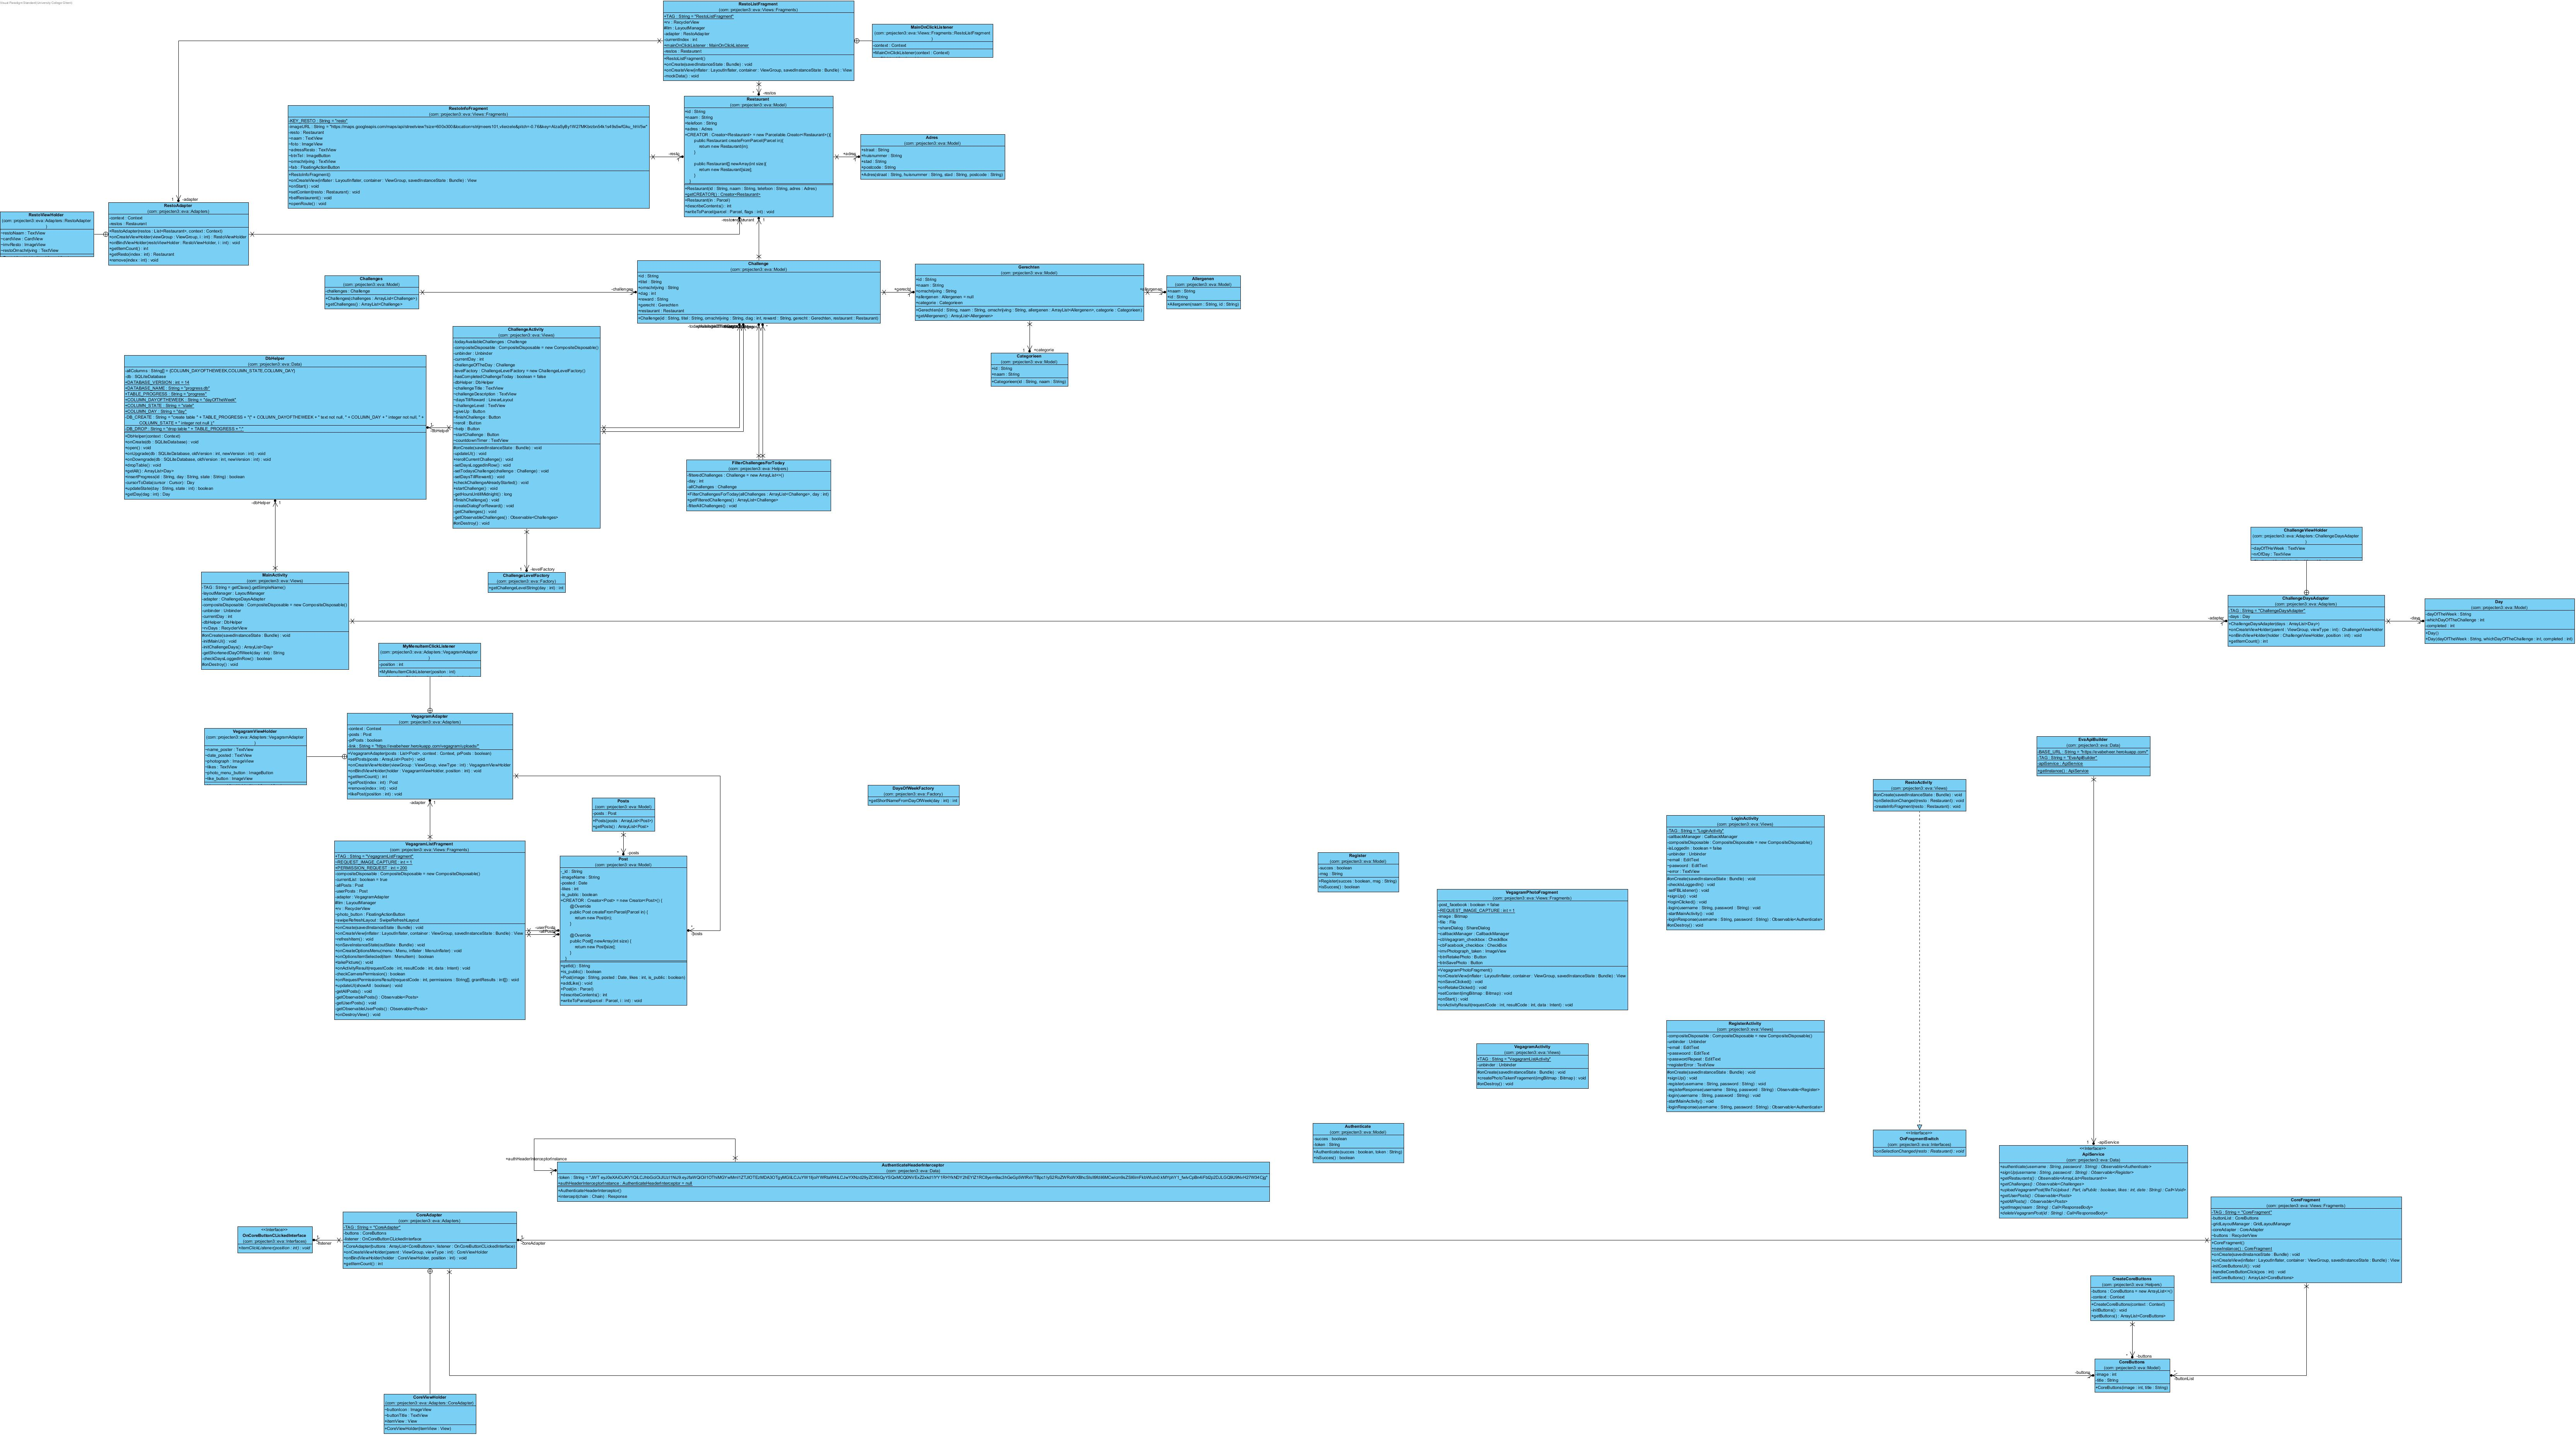
\includegraphics[width=10cm]{img/EvaAndroid.jpg}
	\caption{Eva Applicatie Class Diagram}
\end{figure}

een grote afbeelding is terug te vinden op de GitHub repository via volgende link: 

\section{Deployment Diagram}

Volgende afbeelding toont de deployment diagram aan van de workflow van zowel de Android applicatie als de MEAN applicatie.

\begin{figure}[H]
	\centering
	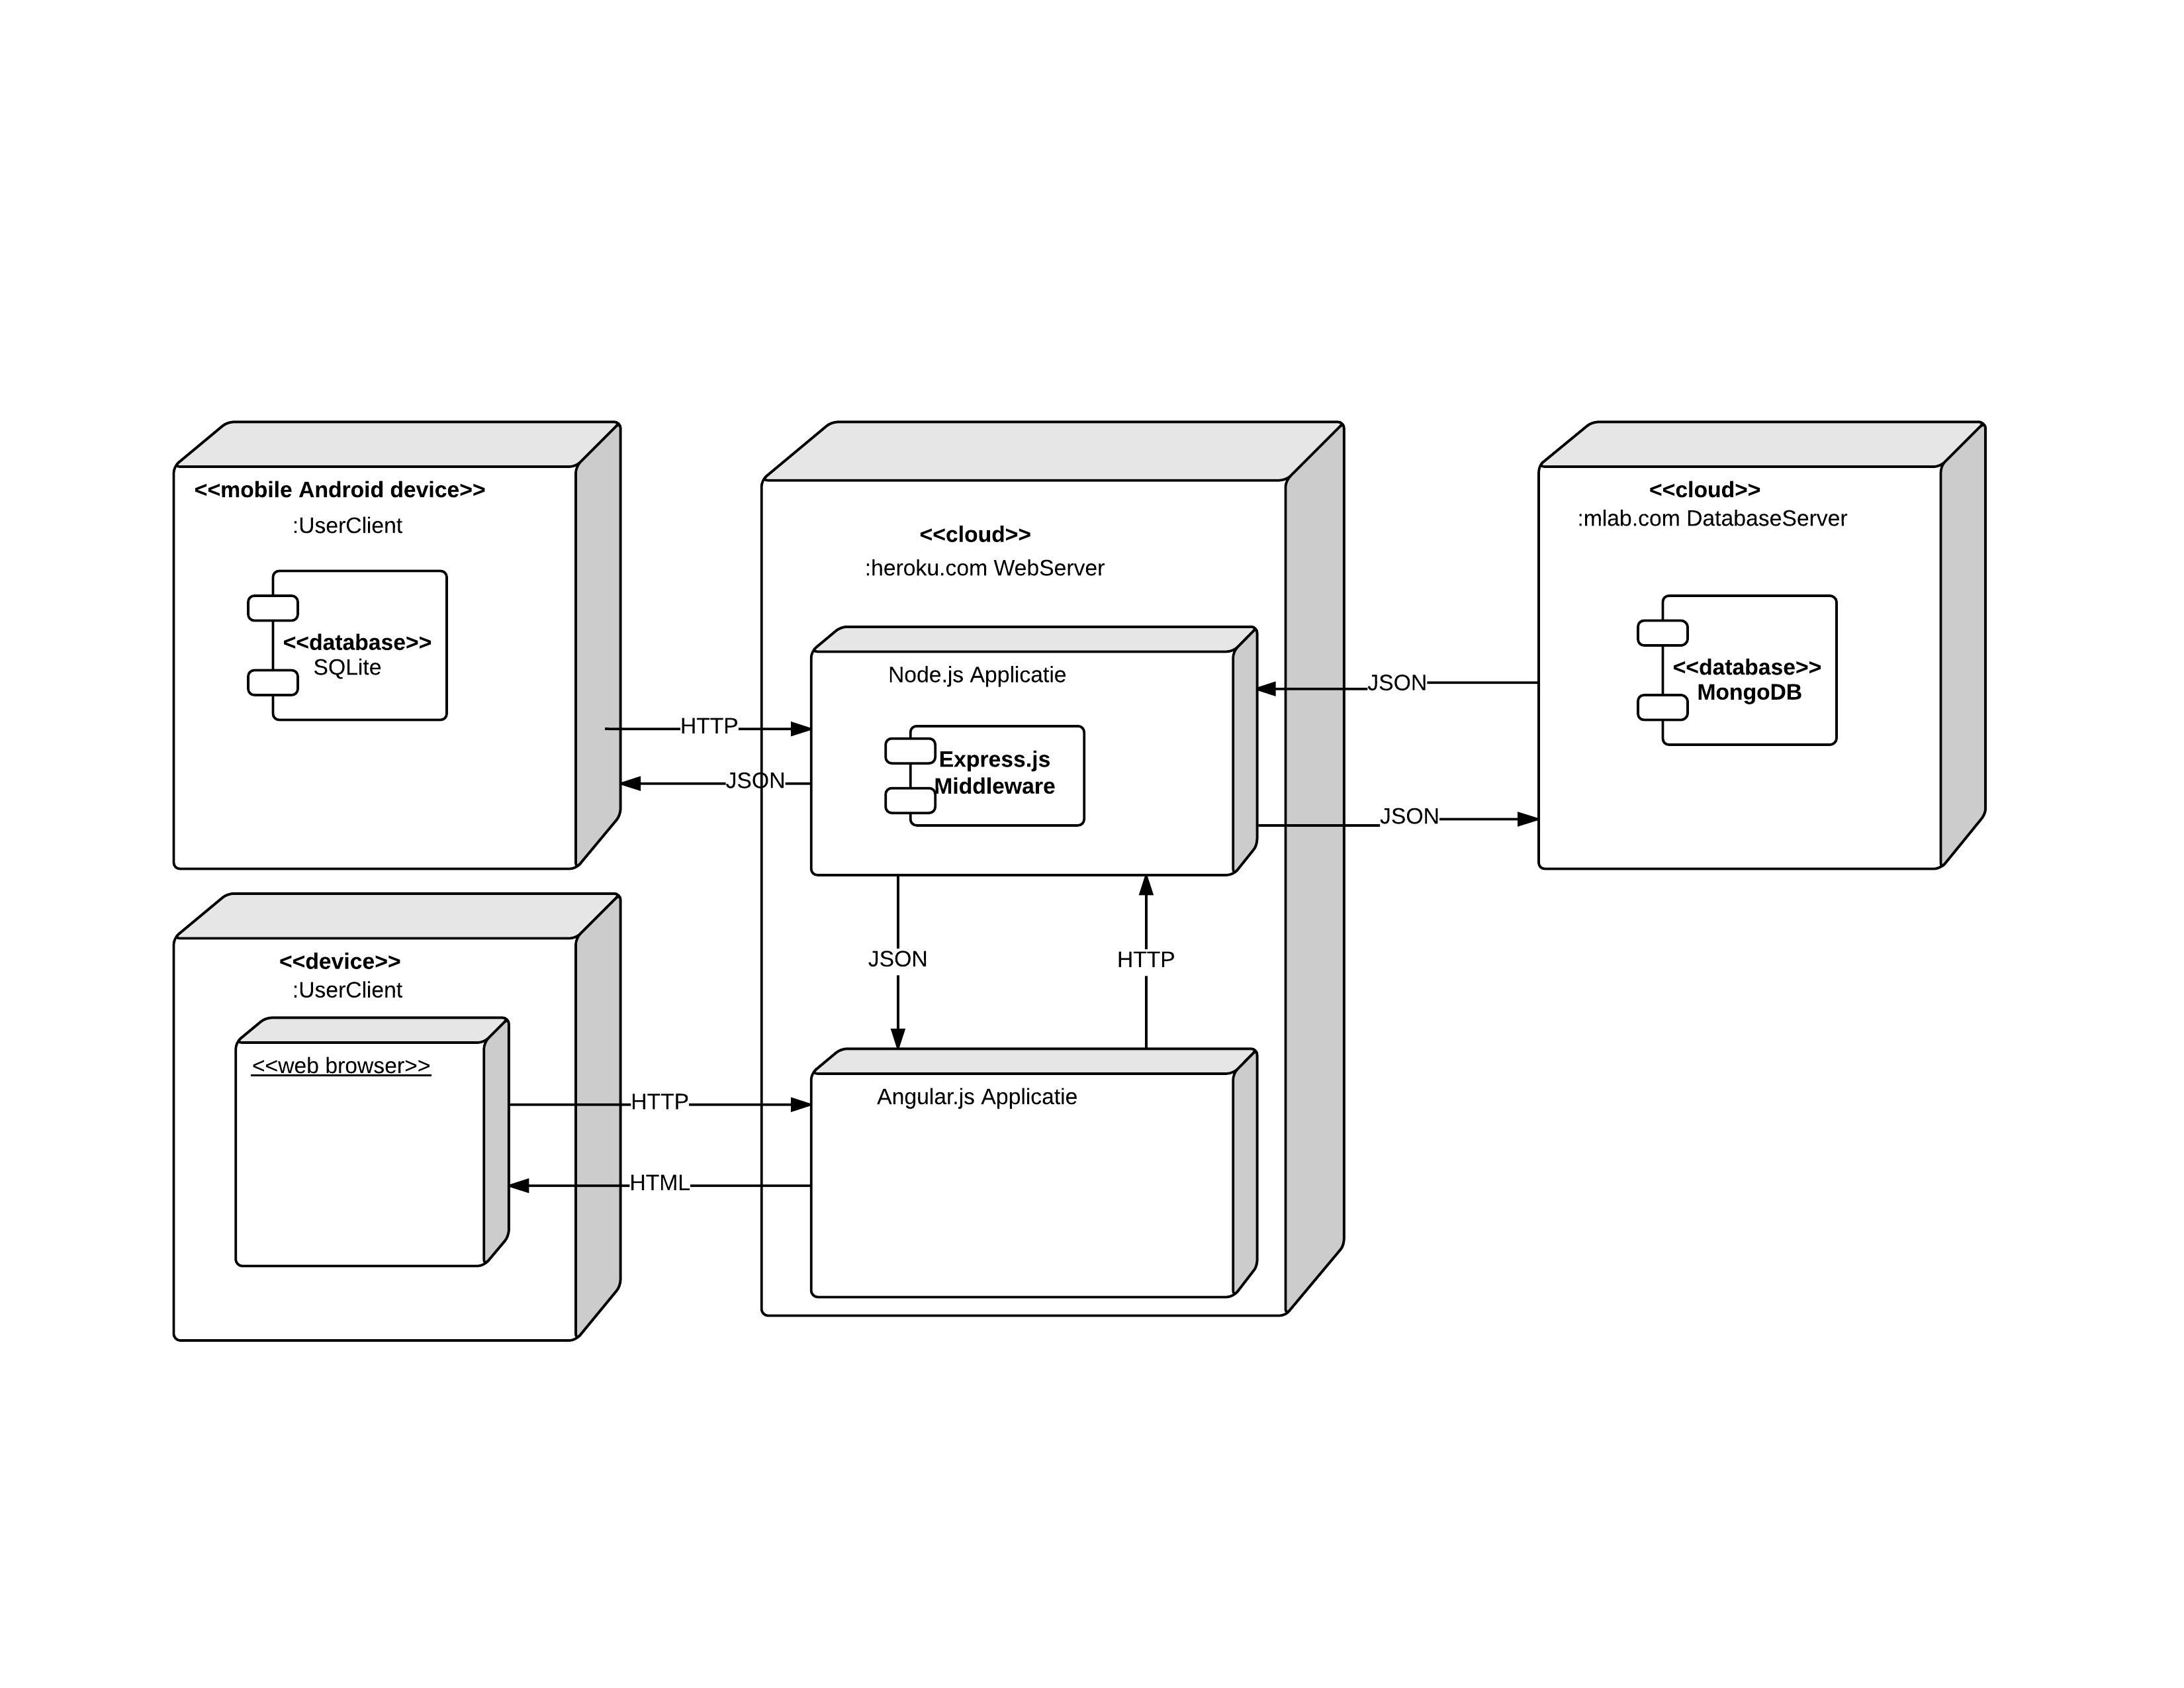
\includegraphics[width=15cm]{img/DeploymentDiagram.png}
	\caption{Deployment Diagram}
\end{figure}

\section{Entity Relationship Diagram}

De volgende afbeelding toont aan hoe het ERD er uit ziet. Waar aan duidelijk te zien is wat de databank van SQLite bevat, alsook de MongoDB.

\begin{figure}[H]
	\centering
	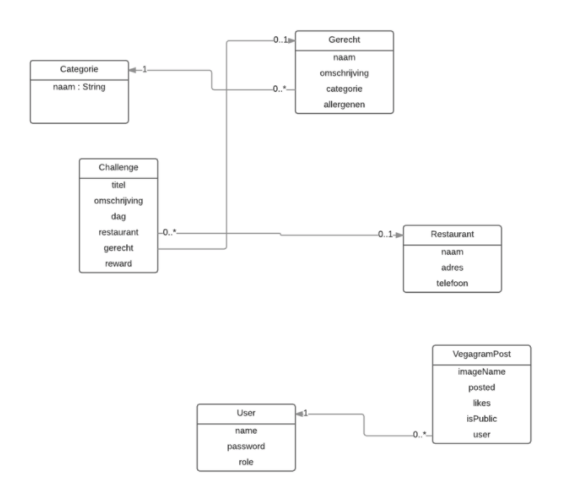
\includegraphics[width=15cm]{img/erd_mongo.png}
	\caption{Entitiy Relationship Diagram}
\end{figure}

De SQLite databank bevat maar één klasse die er als volgt uit ziet

\begin{figure}[H]
	\centering
	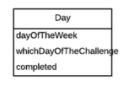
\includegraphics[width=5cm]{img/erd_sqlite.png}
	\caption{SQLite ERD}
\end{figure}

\section{Structuur MEAN}

De structuur van de MEAN applicatie bestaat uit de gevolgde best practices, zo hebben we volgende controllers

\begin{itemize}
\item RestaurantDetailModalController
\item RestaurantModalController
\item authController
\item categorieModalController
\item challengeController
\item challengeDetailModalController
\item challengeModalController
\item gerechtDetailModalController
\item gerechtModalController
\item restauransController
\end{itemize}

Deze maken gebruik van de volgende Factories en services


\begin{itemize}
	\item authService
	\item beheer-factory
	\item challenge-factory
	\item restaurants-factory
\end{itemize}

Dit alles werkt samen om alles te genereren dat getoond wordt in de html van de volgende pagina's

\begin{itemize}
	\item allergenen
	\item categorieen
	\item challenges
	\item gerechtBeheer
	\item restaurants
\end{itemize}

en volgende modals


\begin{itemize}
	\item categorieModal
	\item challengeDetailModal
	\item challengeModal
	\item gerechtenDetailModal
	\item gerechtModal
	\item restaurantModal
	\item restaurantDetailModal
\end{itemize}



\chapter{Best Practices}
\label{ch:bp}

In dit hoofdstuk zijn alle gehanteerde best practices terug te vinden van de twee applicaties. Algemene best practices zijn het gebruik van Github en daarbinnen werken met Git Flow. Zo hebben we voor alle belangrijke use cases een aparte branch aangemaakt die pas op de master branch mogen na dat iemand anders de pull request reviewed.

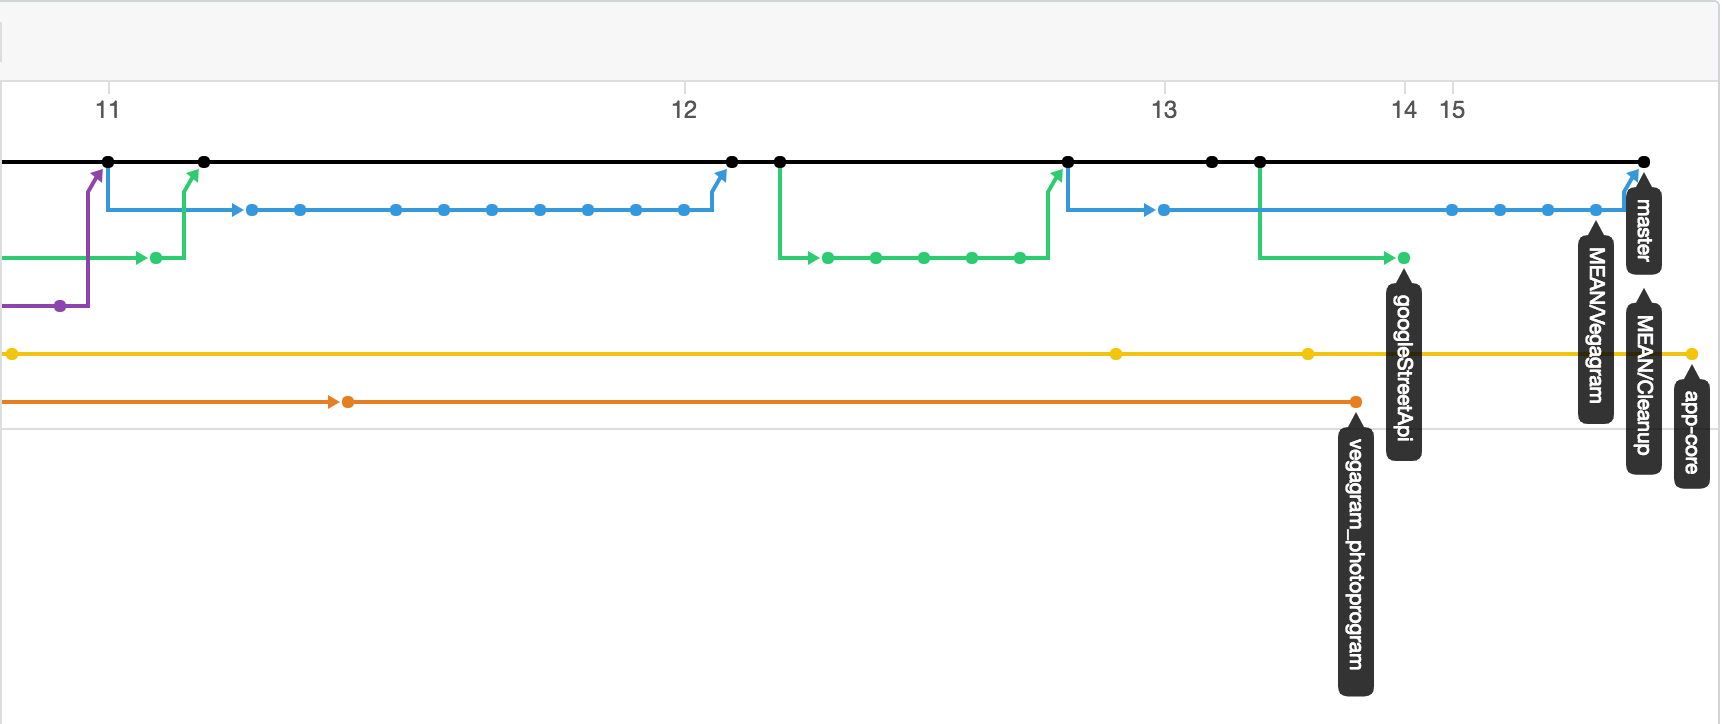
\includegraphics[width=15cm]{img/branches.png}

Als men surft naar:
https://github.com/BramVannevel/eva2017groepH4/pulls?utf8=\%E2\%9C\%93\&q=
is\%3Apr\%20is\%3Aclosed\%20
zijn ook alle gesloten pull requests zichtbaar.

En andere best practice, wat ook aangehaald zal worden in het hoofdstuk met betrekking tot de analyse is onze communicatie. Voor teamcommunicatie hebben we gebruik gemaakt van de handige tool Slack. Hiermee kunnen teams eenvoudig communiceren met elkaar. Slack staat ook toe dat men andere tools integreerd. Zo hebben wij Trello geïntegreerd in Slack waardoor iedereen kan zien wanneer een ticket klaar is. Ook GitHub werd toegevoegd zodat daar direct duidelijk is wanneer een pull request of code review gevraagd werd door een teamlid.

De Trello updates zagen er zo uit

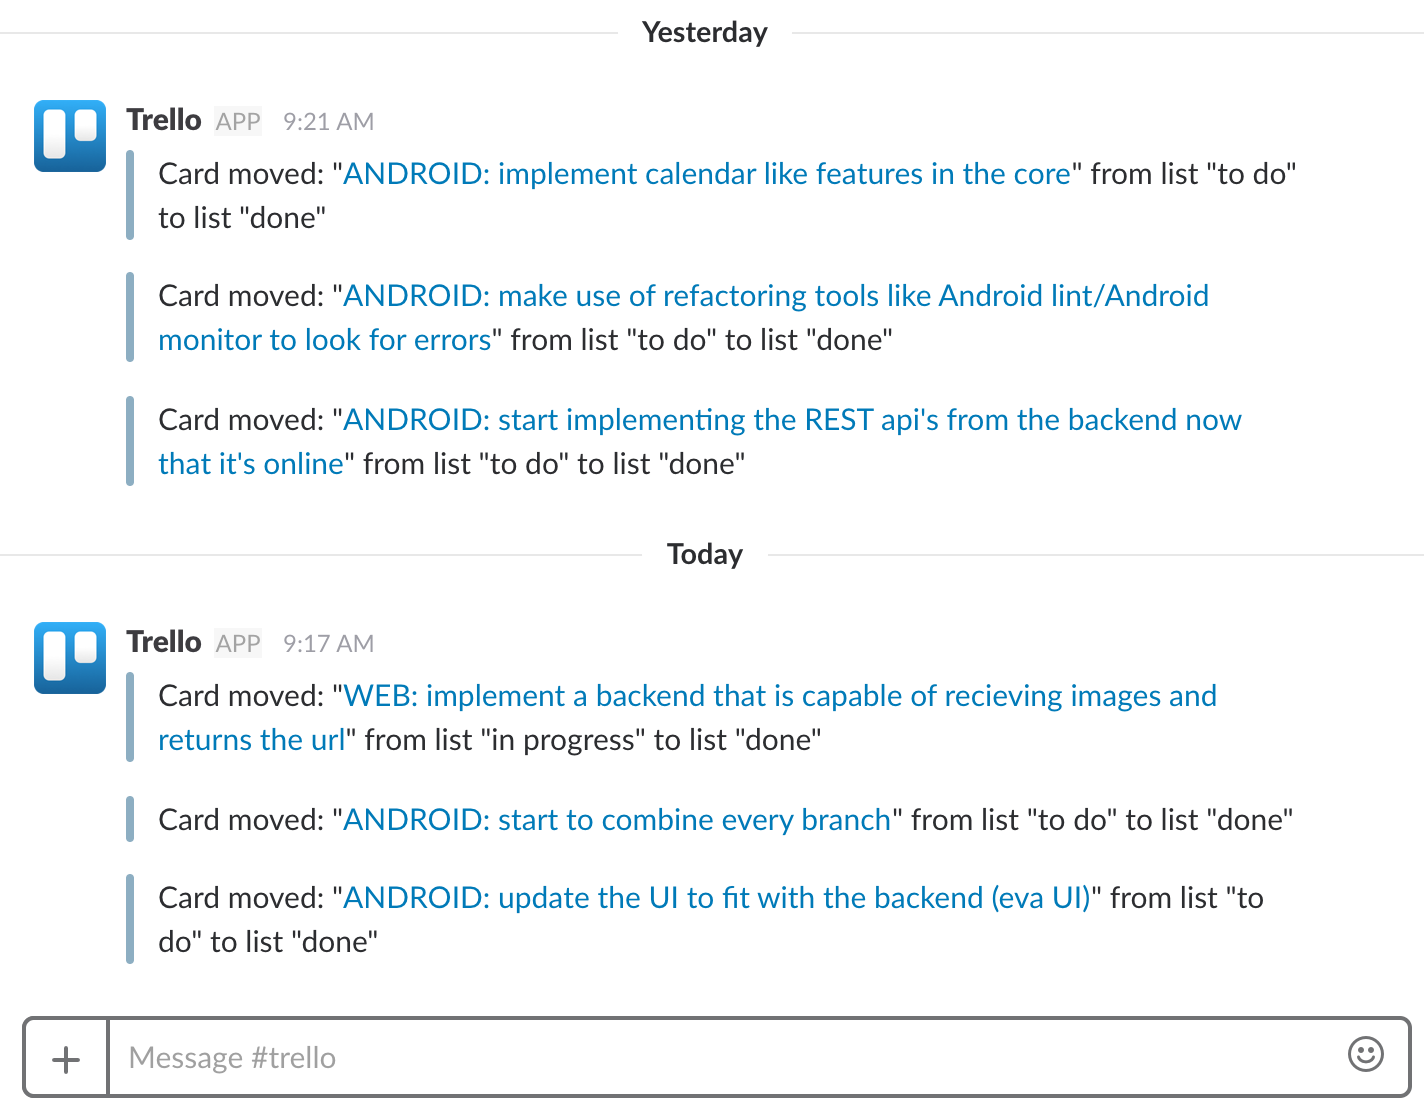
\includegraphics[width=15cm]{img/slack.png}

Binnen slack is het ook eenvoudig om de statistieken te bekijken, zoals hieronder getoond.

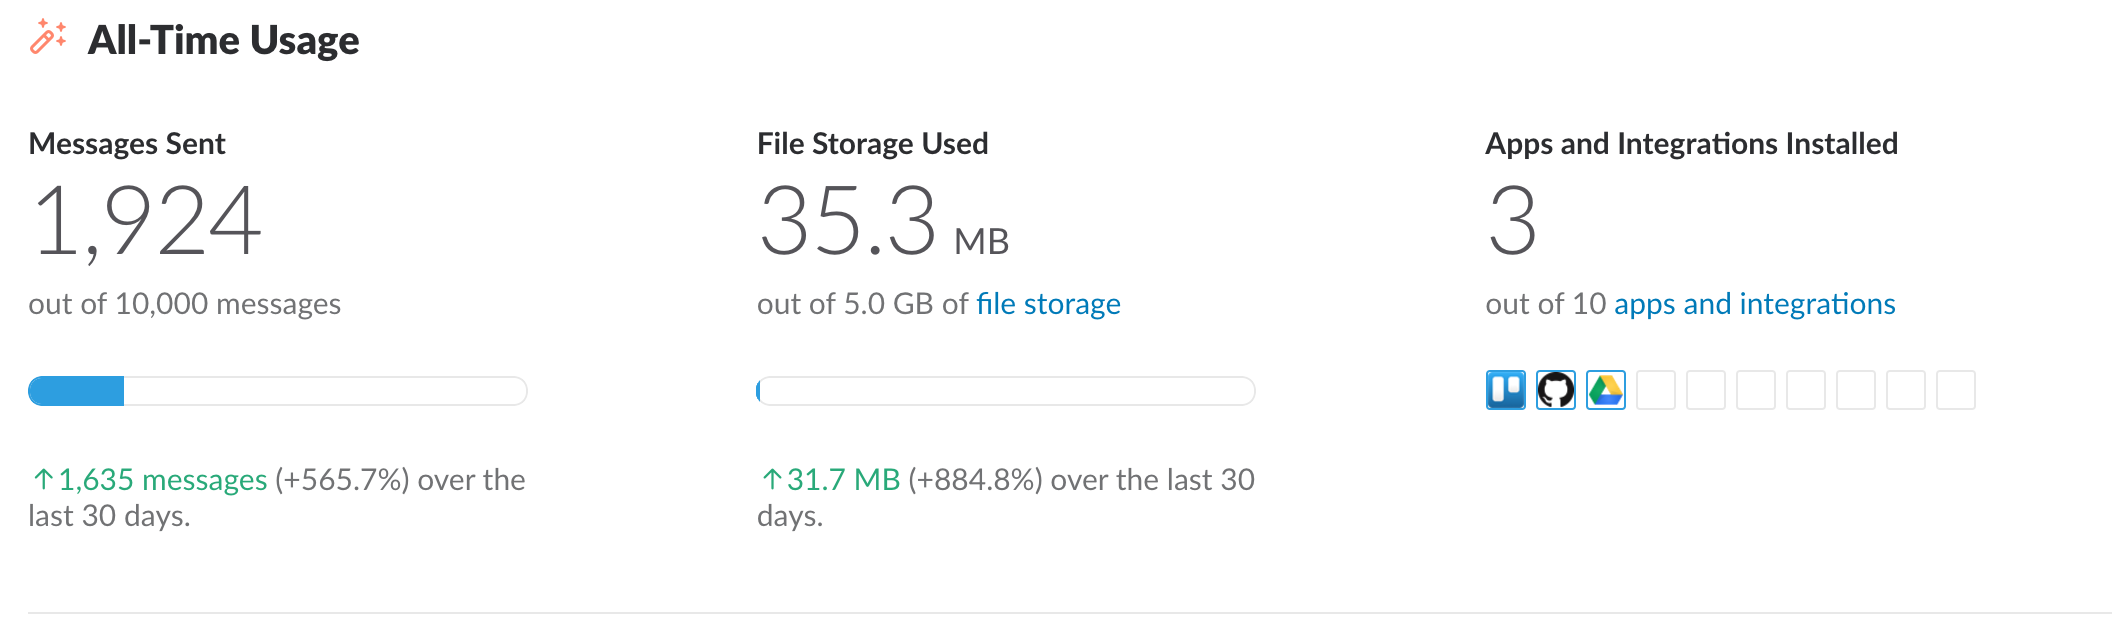
\includegraphics[width=15cm]{img/slack_integrations.png}

Als laatste hebben we ook de scrum en agile principes gerespecteerd en hebben we een scrummaster aangewezen en in iteraties van één week gewerkt per sprint. Dit is allemaal terug te vinden onder het hoofdstuk met betrekking tot de Analyse.


\section{Android}
Binnen Android zijn er veel best practices en normen die gehanteerd en gevolgd kunnen worden om een goede Look and Feel te garanderen voor een app. Zoals het material design. Ook op implementatieniveau zijn er belangrijke verschillen tussen een goede, onderhoudbare app en een minder goede. 

De belangrijkste best practice die achter de schermen gebeurt, maar direct vertaalt naar de user experience van de app is dat alles dat netwerk en databank gerelateerd is asynchroon gebeurt. Voor de netwerk communicatie bekomen we dit door gebruik te maken van OkHttp, Retrofit en RXJava. Dit zorgt voor een asynchrone manier van data ophalen dat perfect in overeenkomst is met de Android Lifecycle van activities en fragments. De reden dat RXJava hierin betrokken wordt, kan het best aangetoond worden aan de hand van onderstaand voorbeeld. 

Als een gebruiker de app opstart en nieuwe uitdagingen ophaalt kan het zijn dat, bijvoorbeeld door het roteren van het apparaat of het openen van een andere applicatie, de activity die de data wil opvragen er niet meer is. Indien men enkel Retrofit gebruikt zal dit leiden tot een crash. Want de asynchrone bevraging zal de data proberen afleveren aan een activity die er niet meer is. Door gebruik te maken van RXJava kunnen we effectief werken met een observer pattern en kunnen activities hun subscriben op data, en als ze destroyed worden unsubscriben zodat de data weet dat ze daar niet naar toe kunnen. Ook heeft RXJava enkele methodes, zoals defer, die kunnen ingeschakeld worden om enkel de data te beginnen opvragen als het effectief nodig is.

Een tweede best practice is het gebruik van een SQLite databank om de gebruiker zijn vooruitgang bij te houden. Zo kan de gebruiker ook offline zijn challenges en vooruitgang bekijken.

Als derde code best practice wordt ook gebruik gemaakt van instancebundles om opgehaalde data in de activity te houden zolang die niet destroyed is. Zo hoeft de applicatie niet altijd een netwerk call te maken als de gebruiker verwisselt van schermen om daarna terug te keren naar het eerste scherm. Zoals bijvoorbeeld het geval is in de Vegagram activity om de posts bij te houden.

Ook wordt veel gebruik gemaakt van fragments zodat een tablet versie ook een makkelijk te implementeren mogelijkheid is. Verder rond UI wordt ook veel gebruik gemaakt van de (relatief) nieuwe ConstraintLayout omdat deze veel performanter is dan RelativeLayout en aanverwanten. Voor het tonen van lijsten gebruikt de applicatie Recyclerviews met als rij een cardview, die opgevuld worden aan de hand van het viewholder patroon. Voor creaties met meerdere mogelijkheden gebaseerd op een input werden meerdere factories geïmplementeerd.

een overzicht van gebruikte patterns:
\begin{itemize}
	\item Factory pattern
	\item Observer pattern
	\item Viewholder pattern
	\item Singleton pattern
	\item Builder pattern
\end{itemize}

kleine, en niet gebruikersgevoelige info wordt opgeslaan in de shared preferences zodat die snel en eenvoudig overal aanspreekbaar zijn, bijvoorbeeld een Json Web Token (jwt). 

Zoals eerder aangehaald is de mappenstructuur ook zeer intuïtief en makkelijk uitbreidbaar bijvoorbeeld om bepaalde classes terug te vinden. Een meer algemene code best practice is ook dat de code zo geschreven is dat ze makkelijk uitbreidbaar en aanpasbaar is. Door middel van factories, interfaces en design keuzes. Een voorbeeld van zo een design keuze is het startscherm. Hier zien we vier knoppen die in een grid terug te vinden zijn. Initieel werden die geïmplementeerd door middel van een TableLayout en dan vier maal hard gecodeerde knoppen in cardviews toegevoegd, maar na een pull request en analyse kwamen we tot het besef dat dit niet uitbreidbaar nog onderhoudbaar is. In de app wordt nu gebruik gemaakt van een Recyclerview met dynamisch gegenereerde knoppen gebaseerd op één klasse die ze kent. Stel dat EVA nog functionaliteit wenst toe te voegen of extra knoppen kan dit op één plaats en wordt alles overal aangepast.


Een laatste best practice is het feit dat er gebruik gemaakt werd van de resource bundles. Zo zitten alle strings in de string resource alsook alle colors. De gebruikte iconen binnen de applicatie zijn afkomstig van de vectors die terug te vinden zijn en gratis te gebruiken, onder de Apache Licentie. Dit heeft als voordeel dat elk icoon op elke smartphone er goed uit ziet.

Binnen Android werken we ook veel met afbeeldingen, zoals de afbeeldingen die kunnen getrokken worden en de Vegagram Posts die getoond worden van andere gebruikers die publiek zijn. De best practice, zoals beschreven in onderstaande sectie, bestaat uit het feit dat geen afbeeldingen direct mee komen via de GET calls. We slaan de afbeeldingen op op de server, en sturen een url naar de afbeelding mee met de call. Dit bespaart tijd (lengte van de duur van de call), geheugen en data van de gebruiker zijn toestel. Daarna kunnen de foto's ingelezen worden via libraries zoals Glide of Picasso en zo door.

\section{MEAN}

Ook voor het webgedeelte werd rekening gehouden met best practices. Zo wordt er gebruik gemaakt van Webpack om alle statische resource bestanden te bundelen. Om de CSS overzichtelijk te houden werd er gebruik gemaakt van Sass. Binnen angular werd de functionaliteit netjes opgesplitst aan de hand van controllers, factories en services en wordt voor de navigatie tussen de verschillende paginas gebruik gemaakt van angular-ui-router. 
Om de verschillende endpoints voor de netwerkoperaties overzichtelijk te houden, werd er gebruik gemaakt van een 
individuele module met constanten. Ook met security werd rekening gehouden. Zo maakt het webgedeelte gebruik van een JSON Web Token 
voor de authenticatie en worden alle wachtwoorden eerst gehashed alvorens ze worden gepersisteerd.
Om ervoor te zorgen dat enkel admins kunnen inloggen in de webapplicatie, werd gebruik gemaakt van gebruikersrollen.
Enkel gebruikers met de rol 'admin' kunnen succesvol inloggen in het webgedeelte. Ook wie van buitenaf (bijvoorbeeld via postman) een 
HTTP request stuurt naar een endpoint dat enkel bedoeld is voor admins, krijgt indien hij dit doet met een account met de rol 'user' een
403 Unauthorized response. Op deze manier blijven alle gegevens binnen het bereik van de juiste personen.

Voor het mongoDB gedeelte hebben we, door dat we werken met afbeeldingen, ook rekening gehouden met de persistentie en efficiëntie van de databank. Zo worden afbeeldingen via een POST als binary opgeslagen op de server zelf (via /uploads/MulterNaamVanDeAfbeelding). Enkel de link naar de afbeelding wordt opgeslaan in de databank. Op die manier blijft deze snel en responsief. En is het mogelij om de afbeeldingen te laden door gewoon de link te gebruiken. Dit heeft ook als voordeel dat er geen afbeeldingen mee gestuurd worden via de GET call van de vegagram posts. Dat zou te veel data verbruiken en te veel geheugen consumeren van de Android applicatie.
\chapter{Analyse}
\label{ch:analyse}

In dit hoofdstuk wordt alles omtrent de analyse uitgelegd en beschreven. 

Voor we begonnen aan de effectieve implementatie werd een backlog gemaakt en hebben we gebruik gemaakt van wekelijkse sprints, die starten op woensdag en eindigden precies zeven dagen later. Sander Brugge nam de rol op zich van scrummaster, hij besliste welke tickets die week werden opgenomen en dan kon onderling beslist worden wie wat deed. Ook besliste hij welke tickets de hoogste prioriteit hadden en wat zeker af moest zijn.

Elke week maakte hij een nieuwe sprint aan in Trello, en zorgde ervoor dat via burndown for Trello de vooruitgang kon bekeken worden en dat er een burndown gegenereerd werd. Elke woensdag op het einde van een sprint hielden we ook een retrospective, om te kijken wat goed ging, wat minder goed ging en wat we gaan doen. Deze zijn allemaal terug te vinden in volgende sectie.

Alle communicatie verliep via de proffesionele team communicatie tool Slack. Aangezien iedereen binne het team relatief ver van elkaar wonen. Voor quality assurance werd gebruik gemaakt van Pull Requests op Github. Waar iedereen commentaar kon schrijven, verbeteringen kon voorstellen of meer uitleg vragen over bepaalde stukken code.

\section{Sprints}

in onderstaande sectie zijn de backlog, burndown en retrospective terug te vinden per sprint. De taken werden onderling verdeeld en besproken via Slack.

\paragraph{Sprint 1}
De eerste week hebben we fysiek samengezeten om de startup te bespreken en te discussiëren wat we van de app verwachten. Na de tijd te hebben genomen om de opdracht te bekijken en te beluisteren, kwamen we tot een algemeen idee. Zoals beschreven in het hoofdstuk plan van aanpak. Op basis van ons idee hebben we een backlog gemaakt met de belangrijkste use cases. Voor ons was het sociale aspect zeer belangrijk. Zo kan een gebruiker inloggen via Facebook en Vegagram posts delen op Facebook om andere mensen aan te zetten tot het gebruik van de app of een veganistische levensstijl.


De backlog van de eerste sprint. Hier is direct zichtbaar dat alles in de backlog gestoken wordt, zowel functionele requirements maar ook niet functionele. Een voorbeeld hiervan is het bespreken van de app. Ook hier moet tijd voor gerekend worden in de sprint.

\begin{figure}[H]
\centering
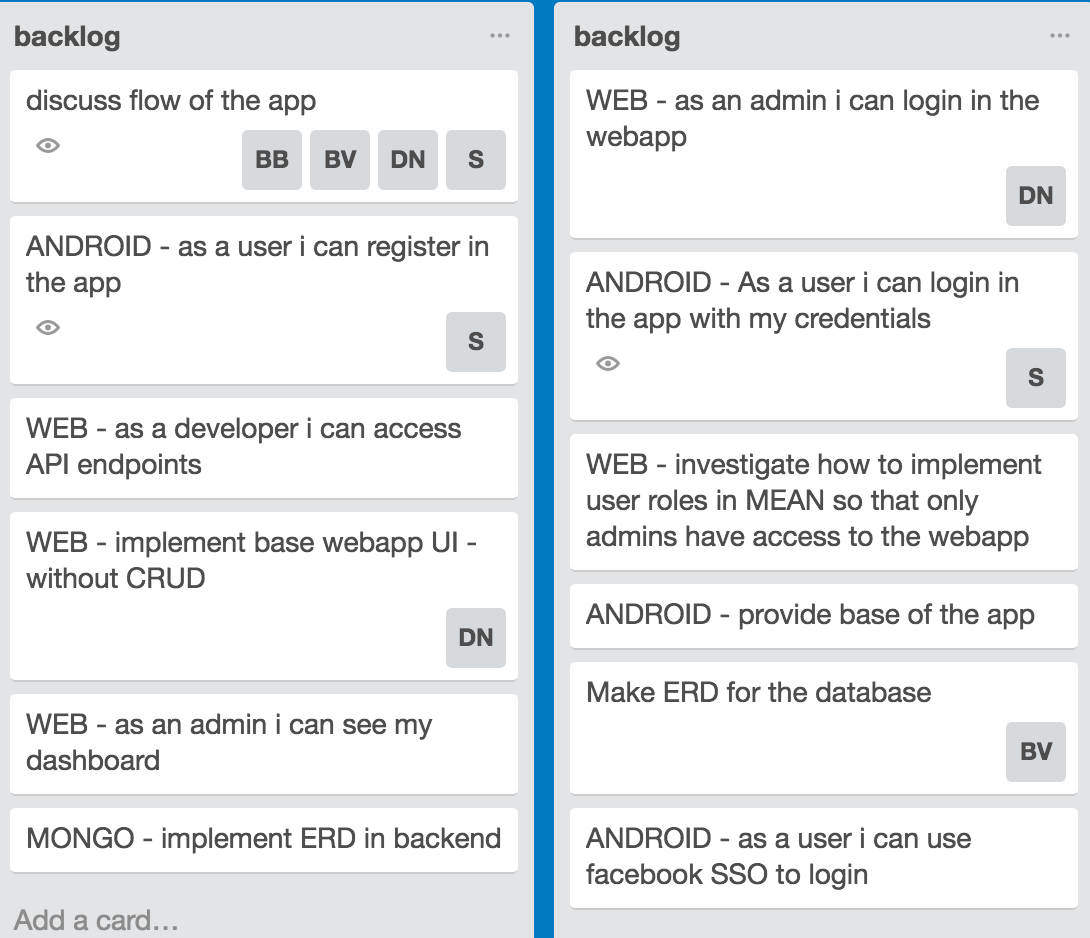
\includegraphics[width=15cm]{img/backlog_week1.png}
\caption{backlog sprint 1}
\end{figure}

De burndown is niet perfect omdat dit de eerste week was en er iets te veel hooi op de vork werd genomen. 

\begin{figure}[H]
	\centering
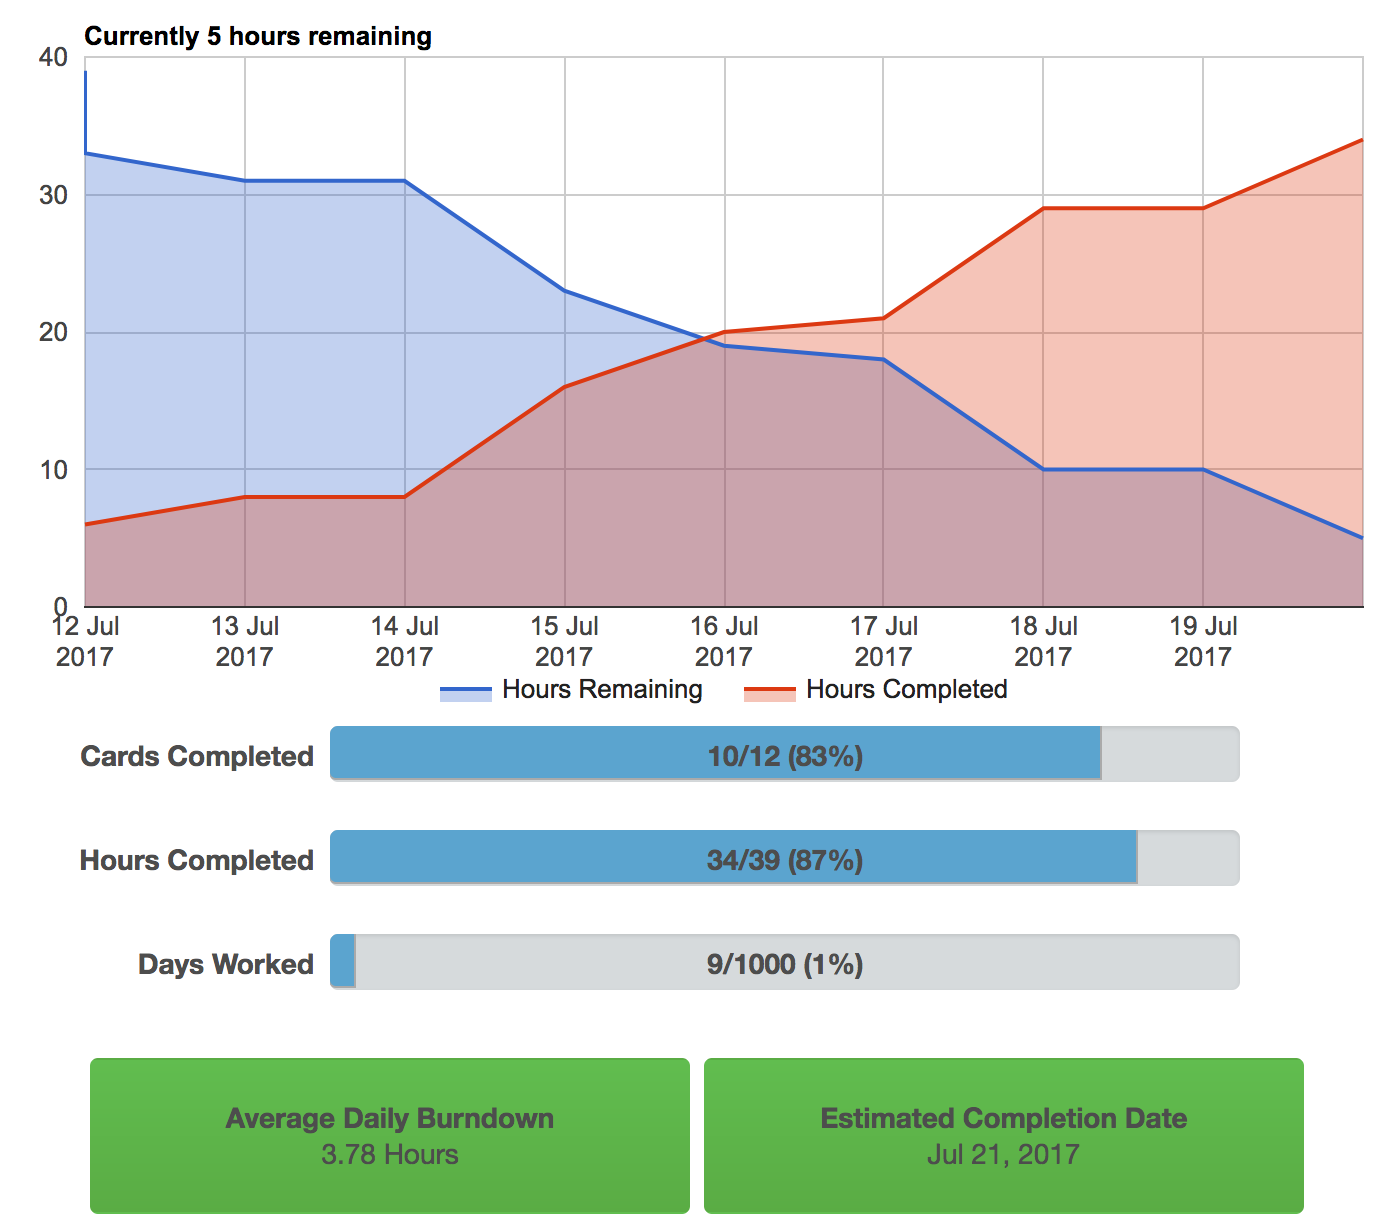
\includegraphics[width=15cm]{img/burndown_week1.png}
\caption{burndown sprint 1}
\end{figure}

Op het einde van een sprint vond ook altijd een retrospective klaar, daarvan is een kort verslag te vinden hieronder.

Sprint 1:
What did we do good

\begin{itemize}
\item Begonnen met goed idee
\item Fysiek samen zitten om het plan te bespreken
\item Vertrokken van uit de basis (ERD/goede afspraken)
\item  Agile werken
\item Best practices respecteren van in het begin
\end{itemize}

What could we have done better

\begin{itemize}
\item Beter inplannen van de tickets
\item Beter verdelen van taken
\item Rekenen op meer tijd voor mooiere UI
\end{itemize}

\paragraph{Sprint 2}
De backlog van de tweede sprint. Dit ziet er op eerste zicht een veel kleinere backlog uit maar de tickets die beschreven zijn waren veel zwaarder en groter van omvang. Hier werd de basis van alles geïmplementeerd dus dit moest ook correct zijn van in het begin.

\begin{figure}[H]
	\centering
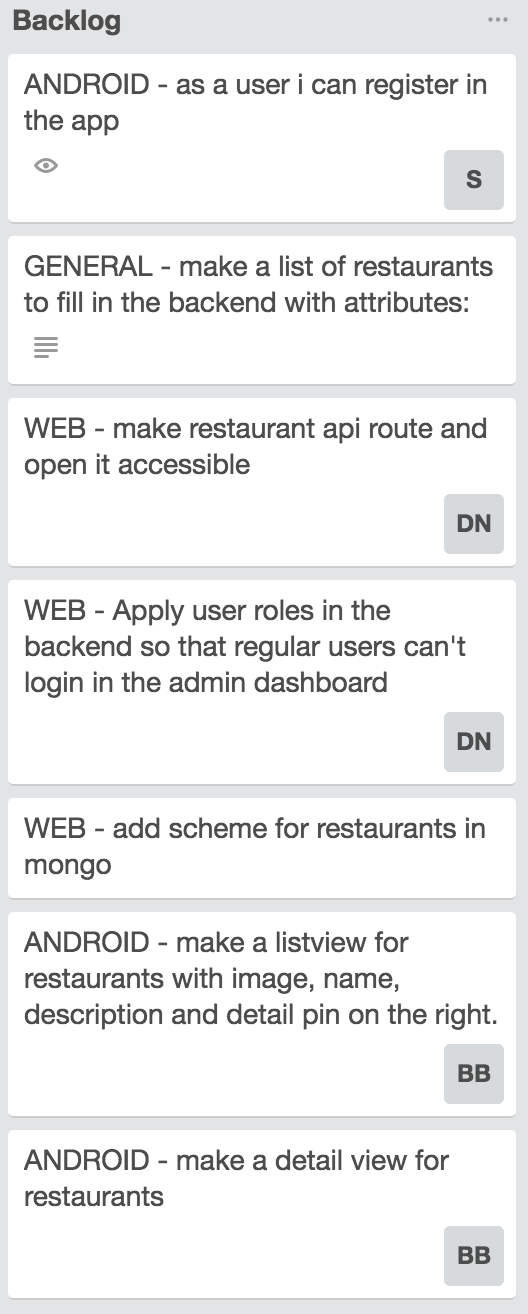
\includegraphics[width=7cm,height=18cm]{img/backlog_week2.png}
\caption{backlog sprint 2}
\end{figure}

Dit ziet er ook al beter ingeschat uit dan de eerste sprint, we maken snel voorruitgang als team!

\begin{figure}[H]
	\centering
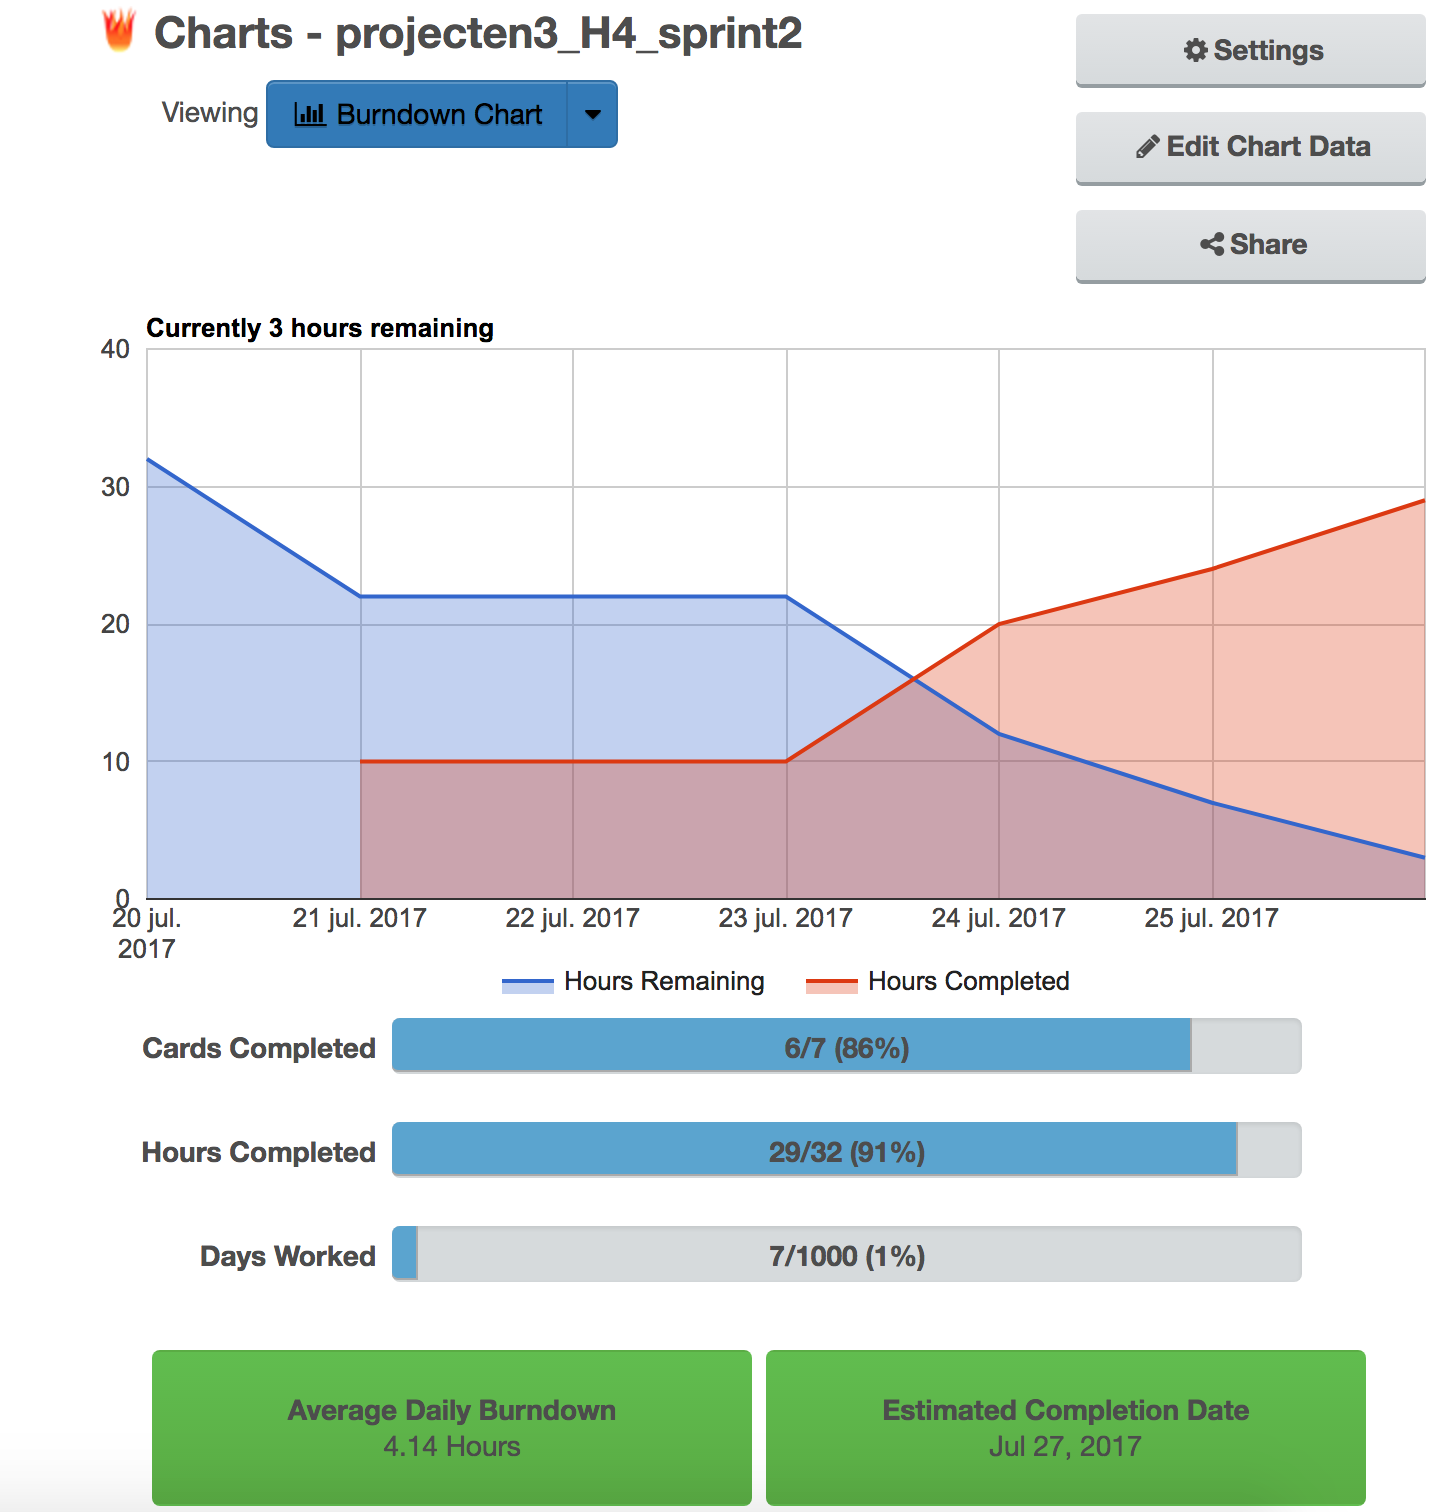
\includegraphics[width=15cm]{img/burndown_week2.png}
\caption{burndown sprint 2}
\end{figure}

Ook hier was na het einde van deze sprint een retrospective, die gehouden werd via Slack.

Sprint 2:

What did we do good
\begin{itemize}
\item met branches werken
\item pull requests om elkaar code te reviewen
\item goed de sprint gepland
\item  goede communicatie dmv Slack
\end{itemize}

what could we have done better

\begin{itemize}
\item betere UI van in begin
\item sommige zaken (zoals properties in pojo's) bespreken in slack ipv in commentaar in de code
\item Javadoc toevoegen test
\end{itemize}


\paragraph{Sprint 3}
De backlog van de derde sprint.

\begin{figure}[H]
	\centering
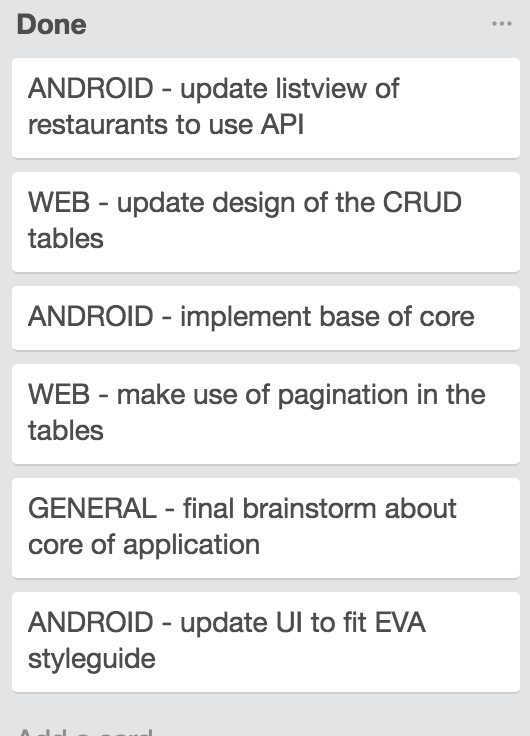
\includegraphics[width=10cm,height=15cm]{img/backlog_week3.png}
\caption{backlog sprint 3}
\end{figure}

Zoals te zien aan de burndown van deze sprint hadden we te weinig opgenomen voor deze sprint. De scrummaster heeft dan beslist dat er extra tickets bij genomen mochten worden. Dit zorgt voor een piek in de grafiek.

\begin{figure}[H]
	\centering
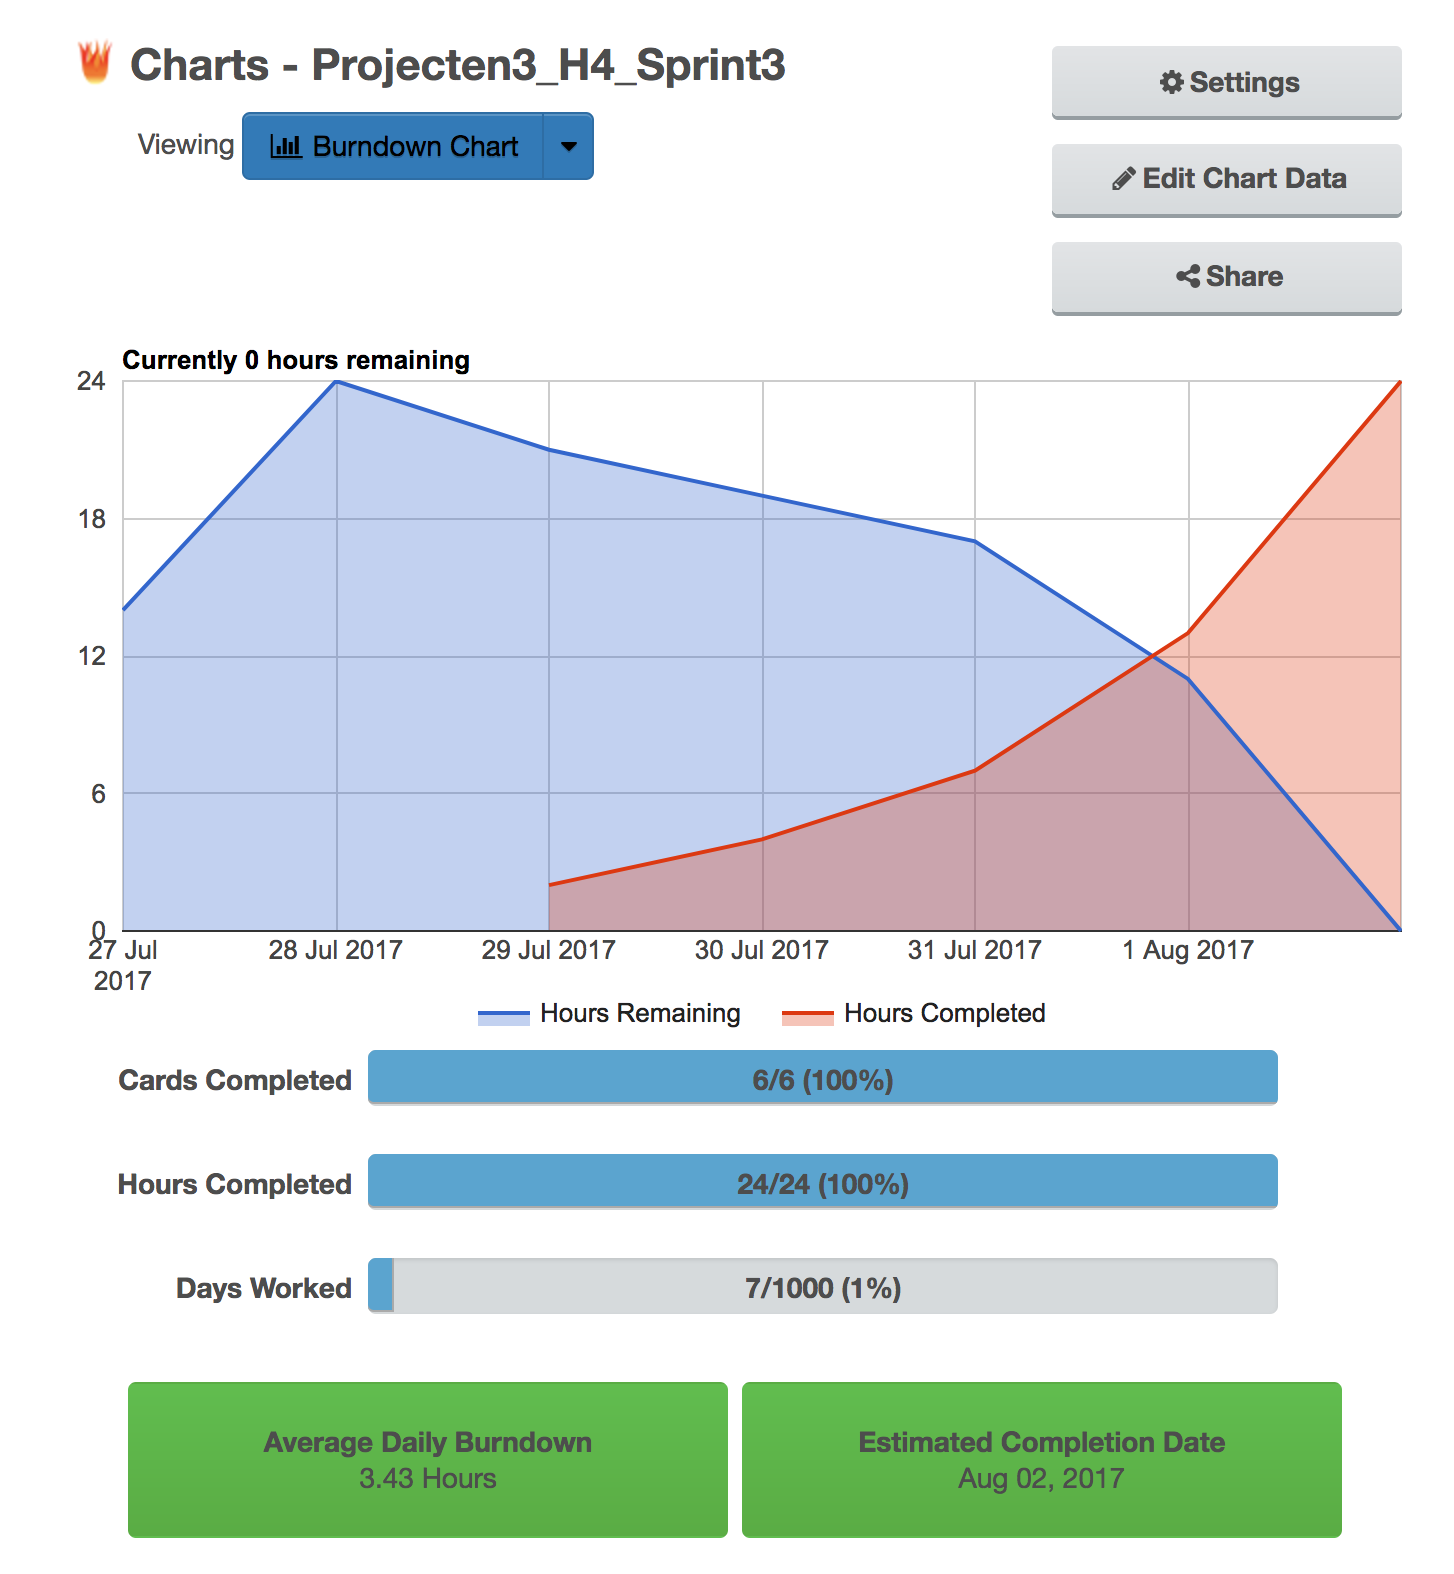
\includegraphics[width=15cm]{img/burndown_week3.png}
\caption{burndown sprint 3}
\end{figure}

Op het einde van de sprint werd opnieuw een retrospective gehouden. Dit zal aanhouden gedurende de volgende sprints ook.

sprint 3:

What did we do good

\begin{itemize}
\item  beter rekening gehouden met de UI en javadoc
\item  coderefactoring van bij de start zodat dat later geen onduidelijke code wordt/blijft
\item verder werken via git flow
\end{itemize}

What could we have done better

\begin{itemize}
\item UI testing
\item unit testing
\item goed webgedeelte en android app laten afstemmen qua properties test
\end{itemize}


\paragraph{Sprint 4}
De backlog van de vierde sprint.

Deze sprint was perfect ingepland en is dan ook tot een goed einde geraakt.

\begin{figure}[h]
	\centering
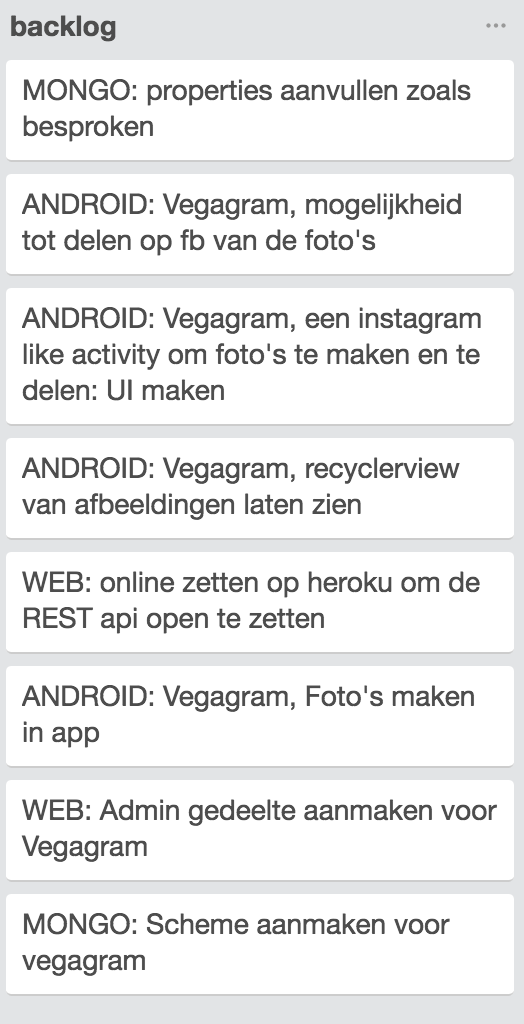
\includegraphics[width=10cm,height=15cm]{img/backlog_week4.png}
\caption{backlog sprint 4}
\end{figure}

Zoals te zien in de burndown ging het werk vlot. Dit is te zien aan de tickets die snel en consistent naar beneden gaan. 

\begin{figure}[h]
	\centering
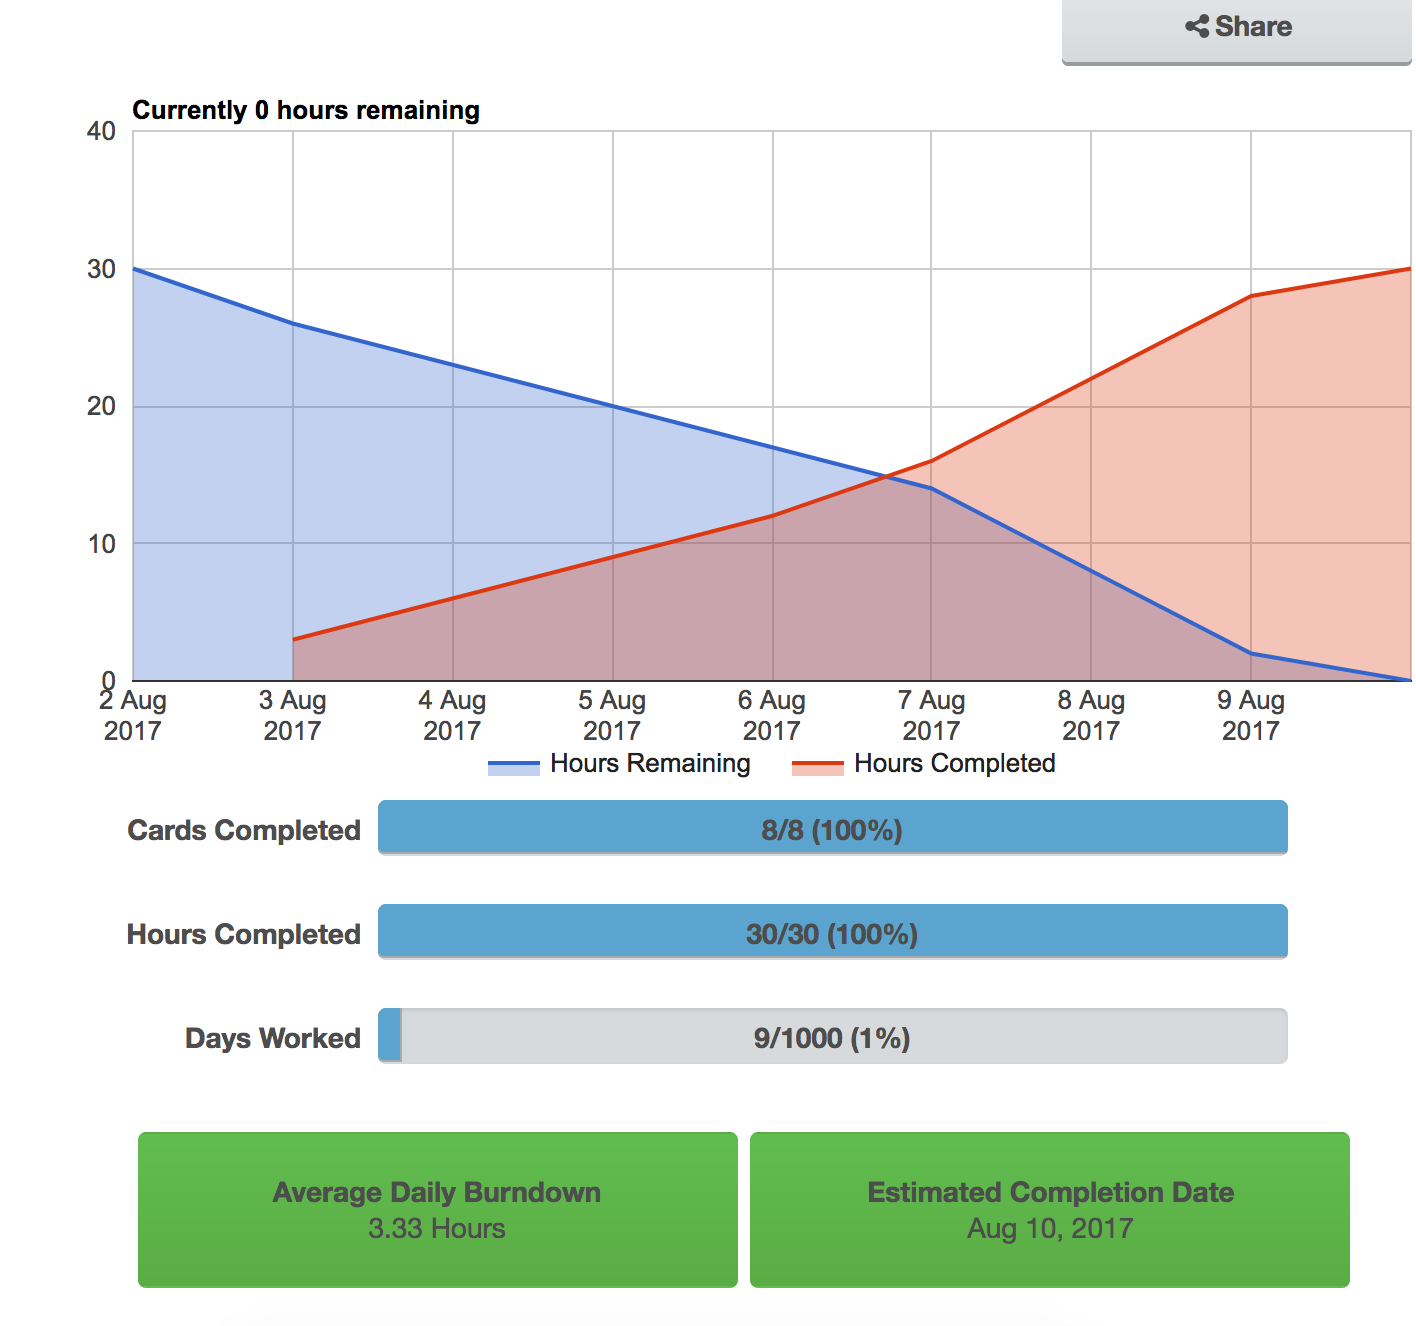
\includegraphics[width=15cm]{img/burndown_week4.png}
\caption{burndown sprint 4}
\end{figure}

Ook hier wordt opnieuw een retrospective besproken.

Sprint 4:

What did we do good:

\begin{itemize}
\item goede communicatie voor backend/frontend
\item coderefactoring van bij de start zodat dat later geen onduidelijke code wordt/blijft
\item pair programming
\item verder werken via git flow
\end{itemize}

What could we have done better

\begin{itemize}
\item UI testing
\item unit testing test
\end{itemize}

\paragraph{Sprint 5}
De backlog van de vijfde sprint.

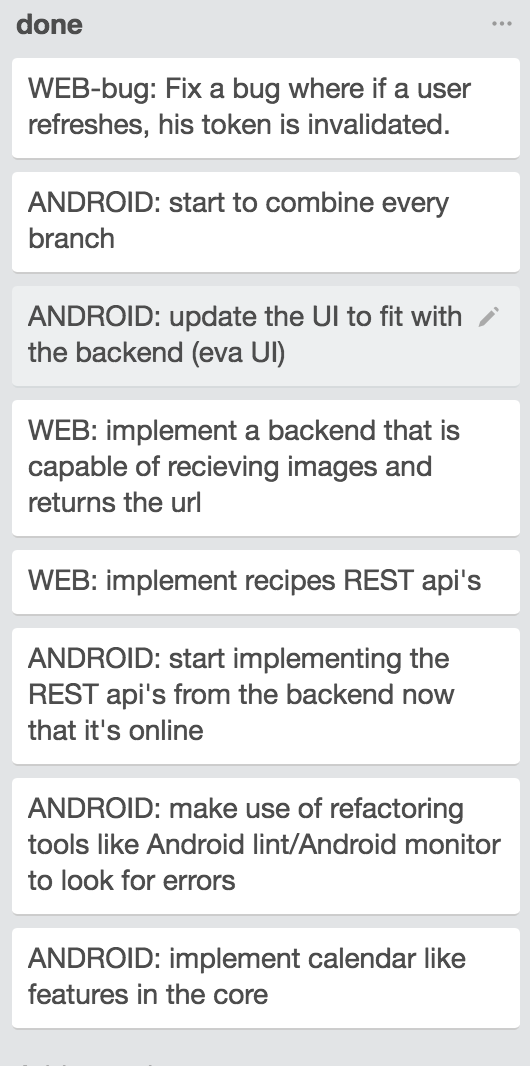
\includegraphics[width=10cm]{img/backlog_week5.png}


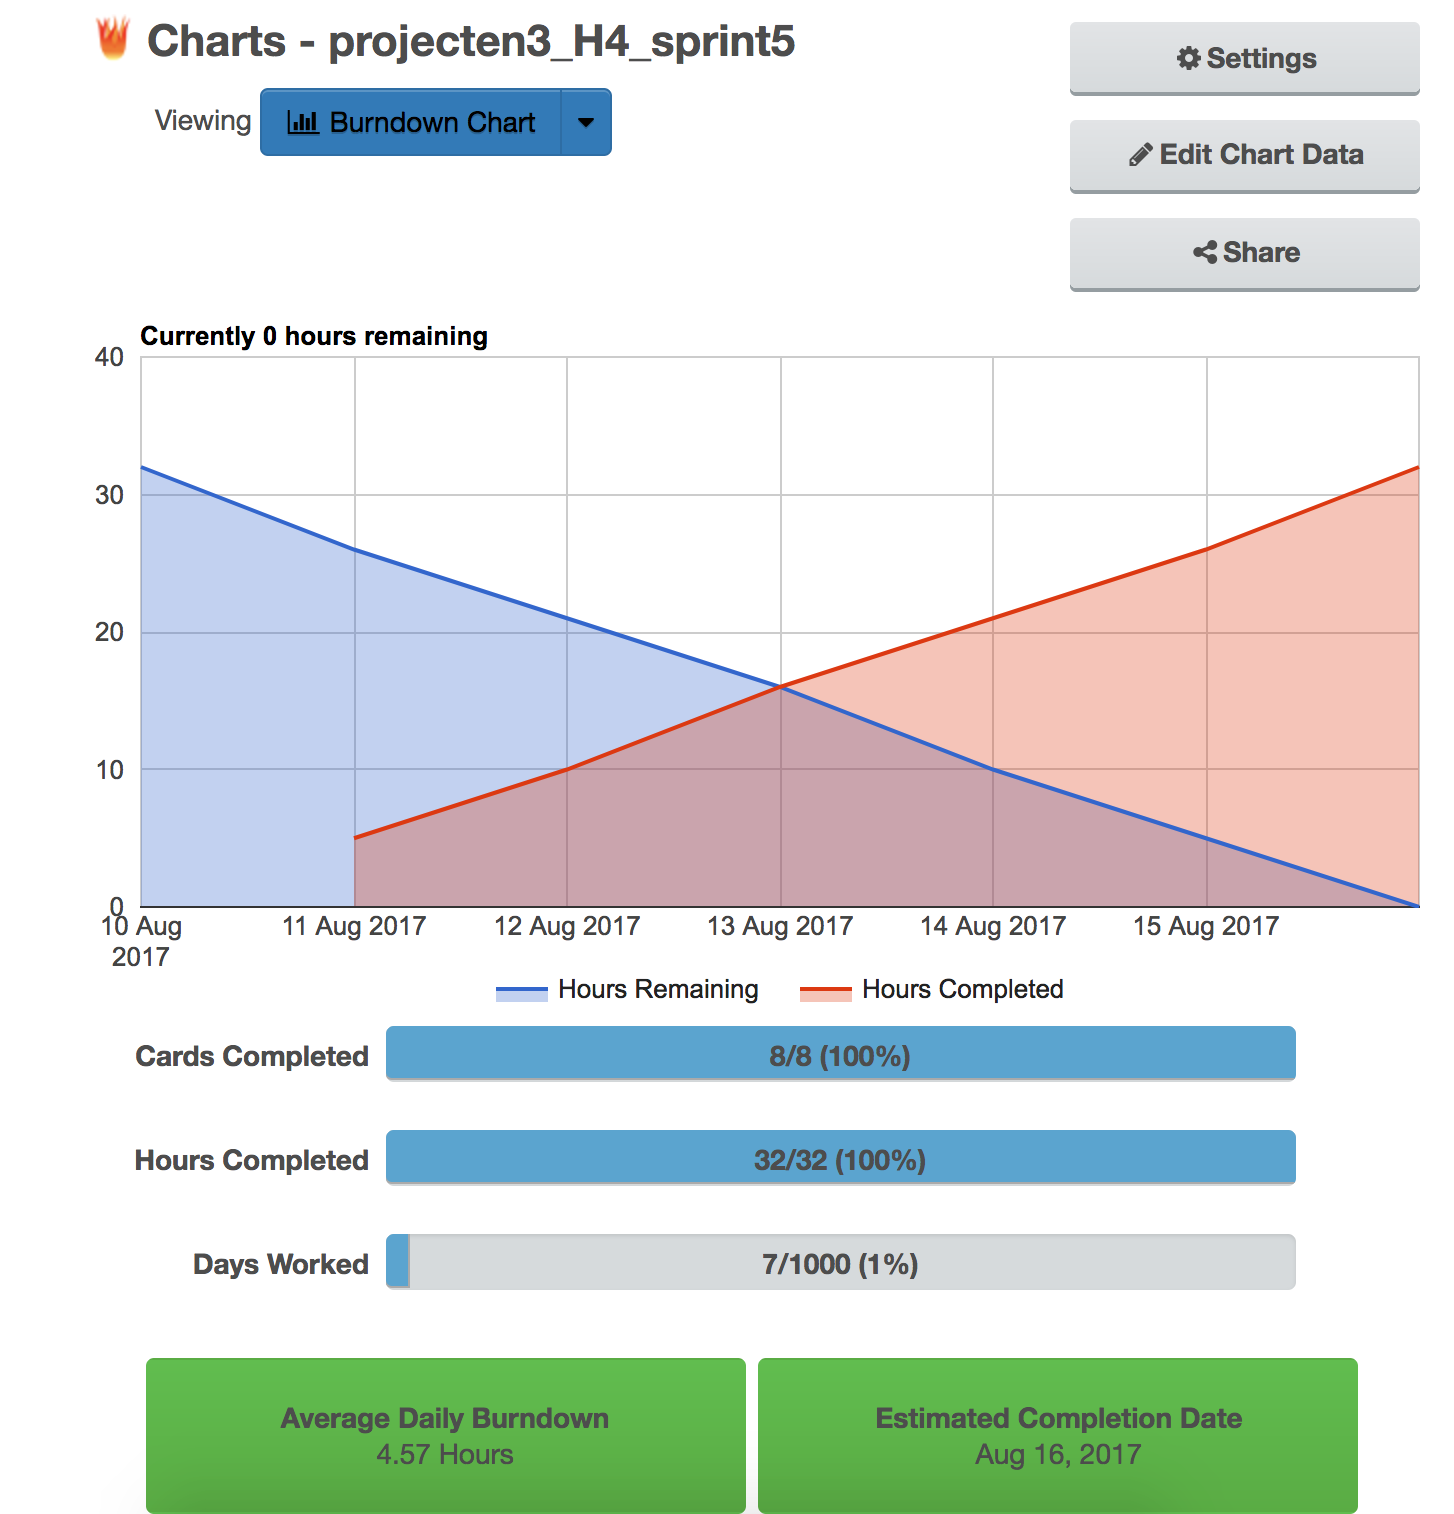
\includegraphics[width=15cm]{img/burndown_week5.png}

sprint 5:

What did we do good:

\begin{itemize}
\item duidelijke taakverdeling
\item mplementatie met best practices in het achterhoofdpair programming
\item verder werken via git flow
\item duidelijke communicatie voor design app in overeenkomst met de backend
\end{itemize}

What could we have done better

\begin{itemize}
\item UI design
\item nog extra javadoc toevoegen
\item beta testing
\end{itemize}

%%---------- Back matter ------------------------------------------------------

\printbibliography
\addcontentsline{toc}{chapter}{\textcolor{maincolor}{\IfLanguageName{dutch}{Bibliografie}{Bibliography}}}


\listoffigures
\listoftables

\end{document}
